\documentclass[a4paper,fleqn,12pt]{cas-sc}

\usepackage[authoryear]{natbib}
\usepackage{tcolorbox}
\usepackage{graphicx}
\usepackage{textcomp}

\usepackage{amsfonts} % 显式加载字体
\DeclareMathAlphabet{\mathbb}{U}{msb}{m}{n}

\usepackage[linesnumbered, ruled]{algorithm2e}
\SetKwRepeat{Do}{do}{while}%
\newcommand\mycommfont[1]{\footnotesize\ttfamily\textcolor{blue}{#1}}
\SetCommentSty{mycommfont}

\usepackage{amssymb} % for empty set
\usepackage{booktabs}
\usepackage{tabularx}
\usepackage{array}
\usepackage{float}
\usepackage[flushleft]{threeparttable}
\usepackage{tabularray} % for better
\usepackage[subsection]{placeins}

\frenchspacing % for consistent spacing between sentences

\newcommand{\killpunct}[1]{} % for reference, remove the comma in the reference of Proceeding

\usepackage{caption}
\DeclareCaptionFont{mysize}{\fontsize{12}{9.6}\selectfont}
\captionsetup{font=mysize}

\usepackage{subcaption}

\usepackage{tabularray}

\usepackage{etoolbox}

% Modify font size of the bibliography
\apptocmd{\thebibliography}{\fontsize{10}{14}\selectfont}{}{}

\usepackage{capt-of}

\usepackage{lineno}

\usepackage{titlesec}
\titleformat*{\section}{\fontsize{12}{20}\selectfont\bfseries}

\usepackage{titlesec}
\titleformat*{\subsection}{\fontsize{12}{20}\selectfont\bfseries}

\SetKwInput{KwData}{Input}
\SetKwInput{KwResult}{Output}

\usepackage{diagbox}
% centering figure and table captions

%%%Author macros
\def\tsc#1{\csdef{#1}{\textsc{\lowercase{#1}}\xspace}}
\tsc{WGM}
\tsc{QE}
\tsc{EP}
\tsc{PMS}
\tsc{BEC}
\tsc{DE}
%%%

\begin{document}
\let\WriteBookmarks\relax
\def\floatpagepagefraction{1}
\def\textpagefraction{.001}
\shorttitle{Preprint submitted to \textit{Elsevier journal}}
% \shortauthors{Lei et~al.}
%\begin{frontmatter}

\title [mode = title]{TranSenti: A spatio-temporal large language model for social media-based analysis of transit satisfaction} 

\author[1]{Da Lei}[%
]

\address[1]{Department of Geography and Resource Management, The Chinese University of Hong Kong, Hong Kong, China}
\address[2]{School of Humanities and Social Science, The Chinese University of Hong Kong, Shenzhen, China}

\author[2]{Shuli Luo}[\%
]

\author[1]{Sylvia He}[\%
]
\cormark[1]


\cortext[cor1]{Corresponding author}


\begin{abstract}
Passenger satisfaction is a key indicator of the success of public transportation systems, necessitating effective measurement methods and data. Although social media data provide a rich source for evaluating passenger satisfaction, its utilization has two primary challenges. First, traditional keyword-based approaches struggle to accurately differentiate between actual passenger experiences and incidental mentions of transit services. Second, generic sentiment models lack domain-specific adaptation to transit contexts, limiting their accuracy in evaluating passengers' transit satisfaction. To address these limitations, we propose TranSenti, a novel framework leveraging Large Language Models (LLMs) with spatio-temporal context for analyzing transit satisfaction from social media. TranSenti employs a hybrid LLM-based filtering mechanism to identify transit-related posts, followed by a fine-tuned spatio-temporal sentiment classification model that evaluates passenger satisfaction by incorporating transit-specific operational context. Experiments demonstrate that TranSenti outperforms state-of-the-art baselines in most scenarios, achieving a 78.1\% F1 score in identifying passenger feedback from raw social media data and 80.8\% F1 score in satisfaction analysis. The findings highlight TranSenti's ability to grasp subtle passenger sentiments by considering real-world transit operational patterns, such as peak-hour service conditions and location-specific issues, eventually supporting data-driven decision-making for transit authorities.
\end{abstract}

\begin{keywords}
large language models (LLMs) \sep social media data \sep spatio-temporal encoder \sep transit service quality
\end{keywords}


\maketitle
\setlength{\parindent}{15pt}
\setlength{\parskip}{0.1in}
\linenumbers

\section{Introduction}\label{sec:introduction}
Public transit systems are the lifeblood of urban life, enabling mobility, economic development, and environmental sustainability \citep{Aguilra2014, zhang2024trafficgpt}. Hence, it is important for transit agencies to understand and improve passenger satisfaction to quantify service quality, inform infrastructure investments, and build long-term loyalty to riders \citep{luo2023influential, susilo2014exploring, de2017travel}. Passenger satisfaction analysis has traditionally relied on techniques such as surveys and focus groups \citep{zeng2024exploring, collins2013novel}. Although such methods have considerable merit, they are frequently subject to constraints such as extensive time and resource costs, periodic data collection with resulting temporal gaps, possible sampling biases, and the risk of retrospective recall bias, in which travelers' memories differ from their actual experiences \citep{luo2023influential, mendez2019using, de2013travel}.

In this context, social media platforms such as Twitter and Weibo have emerged as rich alternative data sources \citep{cheng2025arrival}. These data platforms provide huge volumes of spontaneously generated real-time text that reflects the immediate experiences and sentiments of travelers \citep{collins2013novel, wang2019travel}. Previous research has explored these data using methods such as keyword frequency analysis, topic modeling, and basic sentiment analysis to estimate public opinion of transit service \citep{magnini2011understanding, cheng2011evaluating, collins2013novel}. However, these early approaches often struggled to interpret the complexities of natural language, leading to misinterpretations due to issues like polysemy (words with multiple meanings), contextual ambiguity, and the inability to detect sarcasm \citep{cao2013association, de2017travel, Yan2019}.

Large Language Models (LLMs), such as BERT, RoBERTa, and various GPT models \citep{liu2019roberta, cheng2024recent, lei2025deep}, have transformed the landscape of Natural Language Processing (NLP) at its core. These pre-trained models on large text data sets exhibit unmatched text comprehension, reasoning, and generation capabilities, which make them particularly useful for processing the huge amounts of passenger reviews on social media platforms. Recent efforts investigated LLMs in the transport industry, applying them to tasks such as traffic prediction \citep{li2024urbangpt}, traffic management through participation in base models \citep{zhang2024trafficgpt}, data imputation \citep{zhang2024semantic}, and simulation of vehicle interactions \citep{Li2025}.

Despite these developments, directly applying general-purpose LLMs to transit satisfaction research poses challenges that prevent them from fully realizing their potential. First, distinguishing user generated posts that report personal transit experiences or evaluations from incidental mentions of transit keywords in unrelated contexts remains a difficulty for current LLMs \citep{luo2023influential}. This difficulty often stems from their lack of domain-specific knowledge and understanding of transit-specific contexts. Second, general-purpose sentiment classifiers do not account for critical spatio-temporal factors that strongly influence passenger satisfaction \citep{cheng2025arrival}. Passenger satisfaction is largely shaped by where and when the travel experience occurs \citep{lei2020inferring}. Ignoring this spatio-temporal context can lead to misclassified sentiment and misleading service evaluations \citep{li2024urbangpt,zeng2024exploring}.

% Despite these developments,directly applying general-purpose LLMs to transit satisfaction research poses challenges that prevent them from fully realizing their potential. The two key limitations are as follows:

% \begin{figure}[pos=htbp,width=15cm,align=\centering]
%   \centering
%   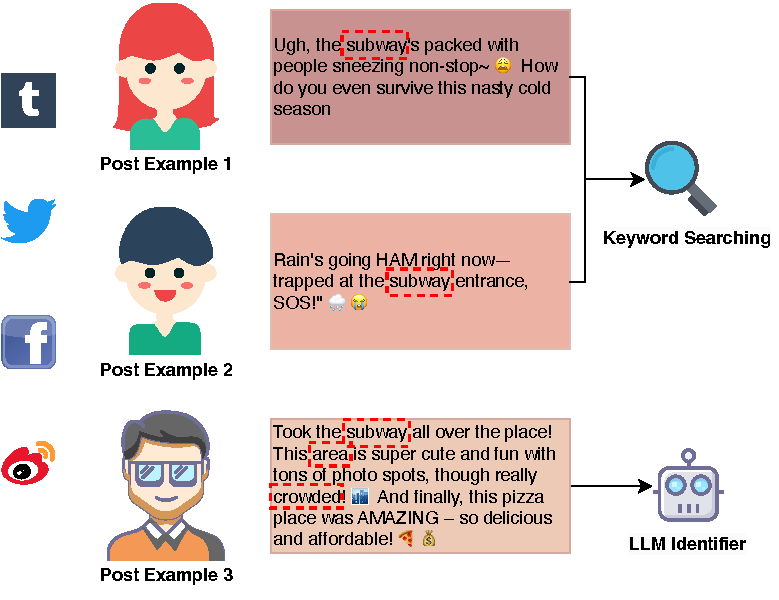
\includegraphics[width=0.7\textwidth]{figs/FilteringMistake.pdf}
%   \caption{Example of transit-related posts filtered by keyword searches and general-purpose LLM methods}\label{fig:FilteringMistake}
% \end{figure}

% First, correctly identifying passenger feedback from raw social media data remains a significant challenge. General-purpose Large Language Models (LLMs), much like earlier methods, can struggle to accurately separate genuine passenger comments---those directly expressing a user's experience or sentiment towards the transit service itself---from incidental mentions where transit-specific keywords appear in discussions of unrelated matters. This difficulty often stems from their lack of domain-specific tuning and understanding of transit-specific contexts. As shown in \hyperref[fig:FilteringMistake]{Fig.\,\ref{fig:FilteringMistake}}, naive keyword searches (e.g., for "subway") or even LLM-based filtering can return off-topic posts. Post 1 uses the metaphorical "subway" in a public health context. Post 2 refers to a "subway entrance" but discusses weather, not transit service. Post 3 is particularly challenging: It contains "subway" and "crowded," but "crowded" describes a photo shoot near the station, not the train or the station itself. These misclassifications introduce significant noise and compromise the validity of sentiment analysis.

% \begin{figure}[pos=htbp,width=15cm,align=\centering]
%   \centering
%   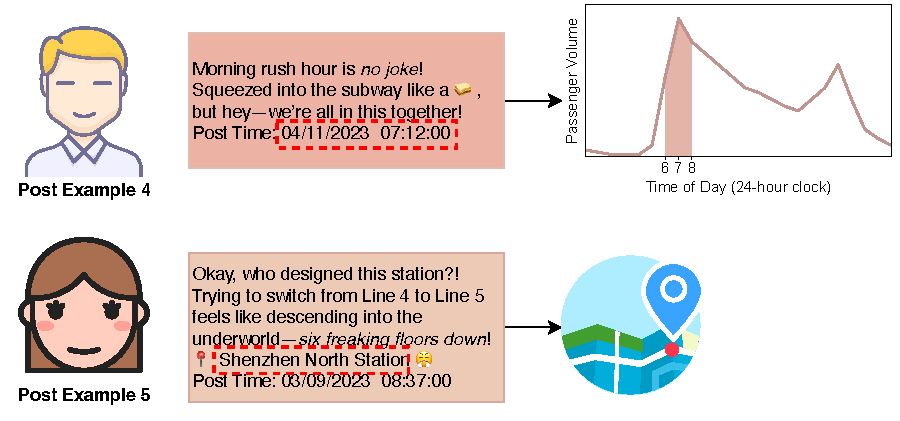
\includegraphics[width=0.7\textwidth]{figs/SpatiotemporalPost.pdf}
%   \caption{Spatio-temporal context in transit service satisfaction analysis}\label{fig:SpatiotemporalPost}
% \end{figure}

% Second, general-purpose sentiment classifiers do not account for critical spatio-temporal factors that strongly influence passenger satisfaction \citep{cheng2025arrival}. Passenger satisfaction is strongly conditioned by the spatio-temporal context of the travel experience \citep{lei2020inferring, luo2023influential}, which means that the expressed sentiment can vary dramatically based on when and where it occurs. For example, as illustrated in \hyperref[fig:SpatiotemporalPost]{Fig.\,\ref{fig:SpatiotemporalPost}}, the overcrowding complaint in post 4, made at 7:12 AM, directly relates to the peak ridership hour during Shenzhen's morning peak. Ignoring this spatio-temporal context, which influences a significant proportion of transit feedback, leads to misclassified sentiment and misleading service evaluations \citep{li2024urbangpt,zeng2024exploring}.

% To address these gaps, we propose TranSenti, a novel framework that integrates LLMs with spatio-temporal contextualization for transit-specific sentiment analysis. Unlike existing approaches, which often rely on traditional keyword-based filtering or generic sentiment models lacking domain-specific adaptation, TranSenti employs a hybrid filtering mechanism. This mechanism combines LLM-driven relevance scoring for semantic understanding, KL-divergence optimization to ensure consensus and reliability across multiple models, and instruction refinement for iterative domain-specific adaptation to identify genuine transit feedback from unrelated social media posts. Subsequently, a fine-tuned sentiment classification model, augmented by a spatio-temporal feature encoder, evaluates passenger satisfaction by explicitly integrating transit context.

To address these gaps, we propose TranSenti, a novel framework that integrates LLMs with spatio-temporal fine tuning for transit-specific sentiment analysis. Compared to existing approaches that rely on simple keyword filtering or generic sentiment models without transit-specific adaptation, TranSenti offers two key innovations. First, it employs a hybrid filtering pipeline that uses LLM-driven semantic relevance scoring, enforces cross-model consensus through a KL-divergence criterion, and iteratively refines instructions to adapt to transit-specific domain language. Second, TranSenti adds a context-aware sentiment model built on a RoBERTa architecture, fine-tuned with an integrated spatio-temporal feature encoder. This model links expressed sentiments to operational conditions such as peak hours or station-specific issues, improving classification accuracy by accounting for spatial-temporal context. We validate TranSenti’s performance in passenger feedback filtering and satisfaction classification compared to state-of-the-art transit sentiment analysis methods with a case study of Shenzhen’s metro system. 

The main contributions of this study include: First, we develop a hybrid filtering framework using LLMs, KL-divergence optimization, and instruction refinement to accurately isolate authentic passenger feedback regarding transit services from incidental keyword mentions in unstructured social media data, substantially improving filtering accuracy over existing methods. Second, we propose a transit context-aware satisfaction evaluation model that leverages a RoBERTa framework, specifically fine-tuned with integrated spatio-temporal transit dynamics. This enables the model to accurately map passenger sentiments (complaints/compliments) to real-world operational patterns (e.g., peak hour conditions, station-specific issues), thereby increasing sentiment classification accuracy by adapting the model to the transit domain. Lastly, we provide a comprehensive empirical validation through a case study in the metro system of Shenzhen with improved accuracy in passenger feedback filtering and satisfaction classification compared to existing state-of-the-art methods in transit sentiment analysis.

The remainder of this paper is organized as follows. \hyperref[sec:liter]{Section \ref{sec:liter}} offers an in-depth review of the literature of relevant studies on the evaluation of transit satisfaction and the application of LLMs in transportation analytics. \hyperref[sec:preliminaries]{Section \ref{sec:preliminaries}} sets the background context of the problem and defines key concepts in relation to satisfaction analysis. In \hyperref[sec:methodology]{Section \ref{sec:methodology}} we present an extended description of the proposed TranSenti framework, including its context-aware satisfaction classification and its hybrid filtering approach.  \hyperref[sec:experiments]{Section \ref{sec:experiments}} describes the evaluation based on real sentiments of passengers expressed in raw posts on social media in Shenzhen, China, and also compares its performance with state-of-the-art methods. Lastly, \hyperref[sec:conclusion]{Section \ref{sec:conclusion}} concludes the key results, discusses implications for the practice of transportation management, and offers future directions in LLM-assisted transportation analytics.

\section{Literature Review}\label{sec:liter}

\subsection{Assessing travel satisfaction using survey and social media data}
The literature on assessing travel satisfaction is based primarily on two main data sources: traditional surveys and emerging social media data. Traditional surveys or questionnarires have long been adopted to collect passengers' ad-hoc travel experience through a series of pre-set questions, usually face-to-face, by mail or online. Its main goal is to quantify passenger perceptions of various service attributes, providing transit agencies with information that can be used for service improvement and strategic planning \citep{he2017impact}. The structured survey design enable detailed examination of specific service aspects, demographic influences, and the effects of interventions on passengers' travel satisfaction \citep{yuan2019ass, pan2024sat}. Key analytical methods include importance-performance analysis (IPA), structural equation modeling (SEM), Bayesian networks, and regression models \citep{luo2023influential}.

These approaches aim to quantify perceptions of service attributes, allowing transit agencies to identify areas for improvement and inform strategic planning. For example, early work by \cite{iseki2010sty} used regression analysis on surveys of 749 bus users in Los Angeles, revealing that frequent and reliable service, along with personal safety, are critical factors beyond physical facility characteristics. Similarly, \cite{ismail2013pas} applied comparative analysis to survey data on passenger preferences across public transport modes in Malaysia, while \cite{cao2017com} employed IPA on 2013 survey data from Guangzhou to highlight differing improvement priorities for bus, bus rapid transit, and subway services. \cite{cheng2018mod} developed a satisfaction model for bus transfers at high-speed rail stations, calibrated via SEM on questionnaires from Xi'an North Railway Station. \cite{wu2016exp} utilized Bayesian networks to quantify the impact of service attributes on overall satisfaction in Nanjing.

The rise of social media platforms has introduced a complementary paradigm for measuring travel satisfaction, offering continuous, real-time, spontaneous feedback from diverse users. This shift addresses many survey shortcomings by providing large-scale data at low cost, with minimal ongoing effort once collection processes are established. Key methods include keyword frequency analysis, topic modeling (e.g., Latent Dirichlet Allocation), sentiment analysis using tools like VADER or TextBlob, and natural language processing (NLP) models such as BERT for advanced text classification. For example, \cite{liu2019nat} used topic modeling and basic NLP on over 25,900 comments about Shanghai's public transport, a scale impractical for surveys, to identify service themes. \cite{mendez2019twi} employed sentiment classifiers to diagnose issues timely among large user bases, outperforming surveys' averaged responses. Similarily, \cite{luo2020urb} used topic modeling and sentiment analysis on Sina Weibo data for Shenzhen subway perceptions, uncovering temporal variations in attributes like congestion and spatial clusters around business districts. A recent work by \cite{alsahar2023twi} applied sentiment analysis and keyword filtering on Twitter to assess responses to bus service changes, linking satisfaction to real-time reliability.

Despite the convincing progress of travel satisfaction measurement on survey data and social-media streams, each source faces certain limitations. For the traditional surveys, they are resource-intensive and typically conducted infrequently (e.g., annually or biennially), yielding outdated snapshots in dynamic environments \citep{liu2019nat}. They are prone to sampling biases from self-selection, which can skew results toward extreme views \citep{rodriguezvale2019imp}, and their structured format restricts responses to predefined options, missing spontaneous insights and real-time fluctuations from operational disruptions or events. In contrast, a key strength of social media is its capacity for precise spatio-temporal linkage, often via geotags or timestamps, along with the potential to reveal unexpected insights through integrated analyses. However, significant gaps persist in social media-based transit satisfaction analysis. A primary challenge is accurately identifying relevant posts from noisy and unstructured textural content \citep{alsahar2023twi, liu2019nat}.

\subsection{Advancement of Large language models in travel satisfaction measurement}
The inherent limitations of traditional survey methods, as well as the continuing challenges faced in using social media data for transit satisfaction analysis, especially in terms of accurate content filtering, emotion-interpretation in specific fields, and spatio-temporal contextualization, highlight the need for more advanced analysis tools. This is precisely where Large Language Models (LLMs) emerged as a groundbreaking solution with abilities in natural language understanding, generation, and reasoning that can directly fill the above-mentioned research gaps \citep{liu2025trip}.

The application of LLMs in transportation research is a rapidly emerging field. \cite{syed2024ben} evaluated the ability of state-of-the-art LLMs to solve traffic engineering problems, evaluating their accuracy, consistency, and reasoning behavior. More directly related to travel behavior, \cite{mo2023lar} proposed using LLMs to predict travel behavior, especially travel mode selection. \cite{jonnala2025exp} explored the potential of LLMs to optimize route planning, reduce waiting time, and provide personalized travel assistance within the San Antonio transit system. A comprehensive review by \cite{yan2025lar} summarizes the methods and applications of LLMs in transportation research, emphasizing their ability to process unstructured textual data to advance development in areas such as travel behavior prediction and general travel queries, and identifies key research gaps and future opportunities in integrating LLMs with existing methods.

There are also several recent studies exploring the potential of LLMs in travel satisfaction analysis. \cite{zheng2023cha} provided an early vision of how LLMs could revolutionize intelligent transportation systems, highlighting their ability to comprehend context, infer intent, and process nuanced language, far beyond the capabilities of traditional keyword filters or rule-based sentiment analysis. This advanced understanding directly tackles the problem of accurately identifying transit-relevant posts. \cite{feng2024eva} introduced an innovative method for evaluating tourism service quality using LLMs and sentiment analysis of travelogue data, emphasizing LLMs ability for "nuanced sentiment recognition at the aspect level." LLMs could also offer an approach to integrate spatio-temporal characteristics more deeply into transit satisfaction analysis. \cite{ruan2024twi}, for example, introduced a framework utilizing LLMs to infer mentioned travel modes from social media posts and to infer people's attitudes toward the associated travel mode, demonstrating the ability of LLMs to understand spatio-temporal mobility contexts.


Despite these promising advancements and the advantages of LLMs in handling complex textual data and performing nuanced sentiment analysis, a significant research gap remains: General-purpose sentiment LLMs, such as Twitter-trained BERTweet or included in TweetNLP, typically are standalone text, lacking the ability to deal with the transit operating context \citep{camacho2022tweetnlp}. They cannot inherently differentiate between opinions expressed during a system-wide failure and those expressed on an ordinary operating day; In addition, they cannot link complaints about delays to known problems happening on a particular transit line or at a specific time. This lack of contextual background can lead to misinterpretations and a false assessment of general service quality, as conceptually illustrated in \hyperref[fig:GeneralVsSevice]{Fig.~\ref{fig:GeneralVsSevice}}. The figure illustrates the typical drop in sentiment classification accuracy (e.g., Macro F1 score) when general sentiment LLMs are applied to transit-specific posts compared to their performance on general social media posts, highlighting their disadvantage without domain-specific fine-tuning. The performance difference observed indicates that models without spatio-temporal features cannot address transit-specific feedback adequately in comparison to their performance on general social media posts. Hence, there is a need to develop sentiment analysis models that could address the interaction between textual sentiment and dynamic spatio-temporal features of the transit network \citep{lei2020inferring, cheng2025arrival}.

\begin{figure}[htbp]
\centering
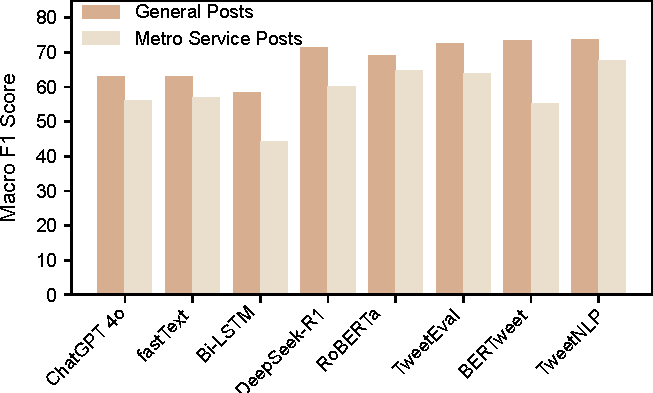
\includegraphics[width=0.8\textwidth]{figs/GeneralVsSevice.pdf}
\caption{Performance gap in sentiment classification between general social media posts and transit feedback}\label{fig:GeneralVsSevice}
\end{figure}

The proposed TranSenti directly addresses these gaps through a hybrid LLM framework that filters service-related posts, and a fine-tuned spatio-temporal RoBERTa model that integrates the contextual information of the transit network to improve satisfaction classification accuracy.

\section{Methodology}\label{sec:methodology}
The proposed TranSenti, as illustrated in \hyperref[fig:overall_framework]{Fig.~\ref{fig:overall_framework}}, is designed to extract insights into transit satisfaction from unstructured social media data. The initial phase, termed as \textit{Data Collection & Preprocessing}, involves gathering raw data from Weibo (and similar social media platforms) and subsequently cleaning them by removing unrelated elements, such as URLs and hashtags. The core of the framework comprises several sequential phases:

\textit{Hybrid Filtering}: This step accepts the preprocessed social media data and implements a hybrid filtering process. It involves an ensemble of Large Language Models (LLMs) fine-tuned with Kullback-Leibler (KL) divergence constraints and prompted with progressively improved directives. The objective is to accurately distinguish and identify posts that actually reflect experiences with transit services from those containing irrelevant references. The output of this phase is a collection of \textit{Filtered Transit-Related Posts}.

\textit{Spatio-Temporal Feature Extraction}: In this step, important contextual information is extracted for every filtered post. Temporal features such as the post's timestamp are retrieved directly, whereas spatial features such as the mentioned station or location are retrieved through geoparsing methods. The output is therefore the text of the post and its corresponding \textit{Time and Location} features.

\textit{Fine-Tuned RoBERTa Model with Spatio-Temporal Encoder}:The input is the text content and spatio-temporal information extracted from the last step. The text is processed using a pre-trained RoBERTa model, and the temporal and spatial information is processed using specialized \textit{Spatio-Temporal Encoders}. These various feature representations are fused together before being passed to the classification layers. This enables the model to learn sentiment within its particular context (e.g., "crowded" during rush hour).

\textit{Transit Satisfaction Analysis}: The last step uses the output of the optimized model to produce \textit{Positive/Negative Satisfaction Scores} for each post. This step yields a quantitative measure of passenger sentiment, allowing the assessment of transit service quality based on both the content of the text and its spatio-temporal context.

\begin{figure}[htbp]
\centering
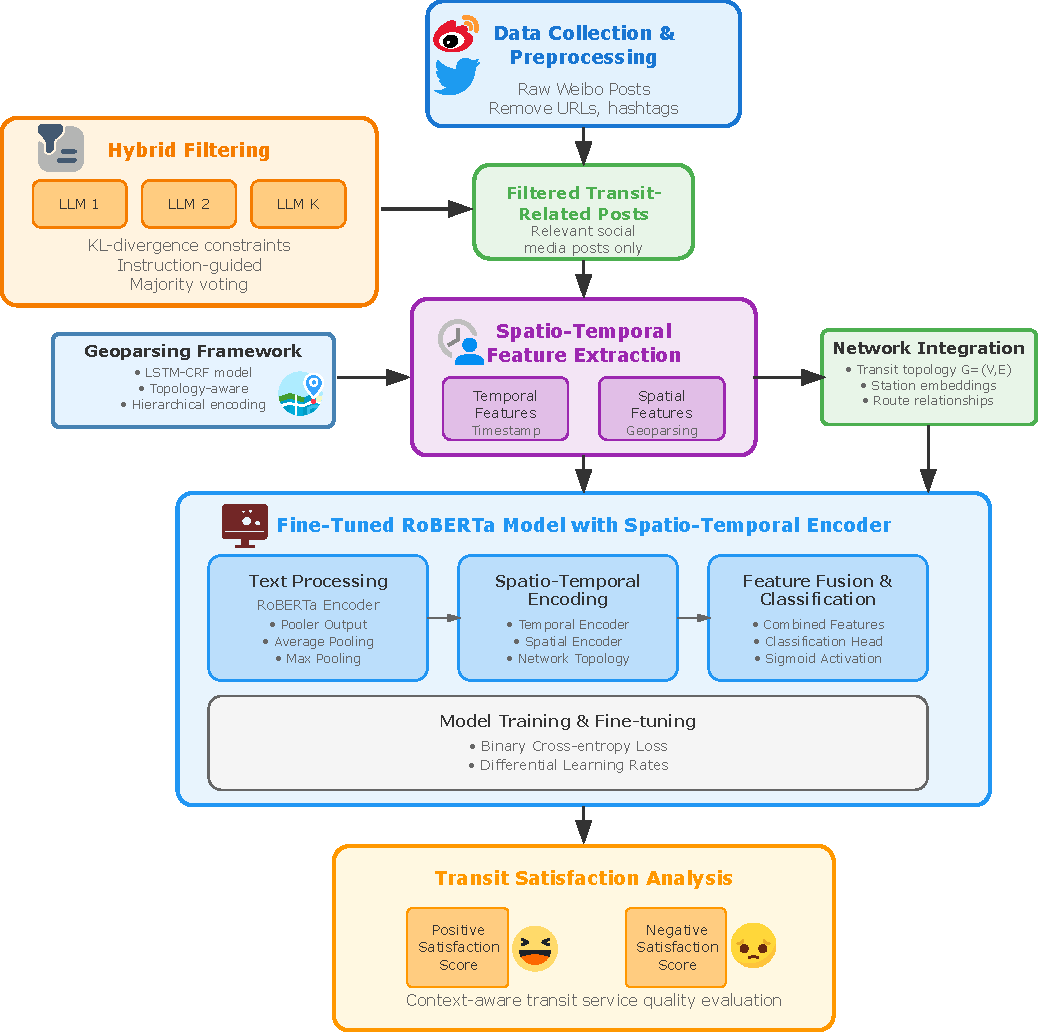
\includegraphics[width=0.99\textwidth]{figs/new_flowchart.pdf}
\caption{TranSenti framework overview}\label{fig:overall_framework}
\end{figure} 

\subsection{Problem modeling}\label{sec:preliminaries}
As mentioned above, TranSenti performs two tasks: (1) extraction of transit-related posts from raw social media streams and (2) evaluation of passenger satisfaction based on filtered messages considering their spatio-temporal context. The components are explained in the following.

Let $\boldsymbol{X} = \{\boldsymbol{x}_1, \boldsymbol{x}_2, \ldots, \boldsymbol{x}_N\}$ denote a collection of $N$ social media posts. Our aim in the process of filtration is to determine what posts refer to real transit service feedback. In a formal sense, we propose a filtration model $\theta$ that classifies each post as relevant or non-relevant:
\begin{equation}
\theta: \boldsymbol{X} \rightarrow \{0,1\}, \quad \boldsymbol{y}\sim\theta(\boldsymbol{y}|\boldsymbol{X}),\quad y_{i}=\theta(\boldsymbol{x}_{i}) = 
\begin{cases} 
1 & \text{if } \boldsymbol{x}_{i} \text{ is about transit service} \\
0 & \text{otherwise}
\end{cases}
\end{equation}
where \(\theta\) is the filtering model that combines LLM-based classification and KL-divergence optimization, $\boldsymbol{y} = \{y_1, y_2, \ldots, y_N\}$ represents the binary relevance labels predicted by model $\theta$.

For every filtered instance \( \boldsymbol{x}'_{i} \in \boldsymbol{X}' = \{\boldsymbol{x}_{i} \mid \theta(\boldsymbol{x}_{i})=1\} \), the satisfaction analysis model $f(\cdot)$ integrates four inputs:
\begin{itemize}
    \item \textbf{Identified post text} $\boldsymbol{x}'_{i}$: Transit-related passenger feedback from social media
    \item \textbf{Temporal context} $t_{i}$: The timestamp of the corresponding post, $\boldsymbol{x}'_{i}$.
    \item \textbf{Spatial context} $l_{i}$: Location extracted via geo-parsing from $\boldsymbol{x}'_{i}$
    \item \textbf{Transit network} $G=(V,E)$: Abstracted topology with nodes $V$ (stations/stops) and edges \(E\) (routes)
\end{itemize}

The satisfaction analysis model $f(\cdot)$ returns independent sentiment scores for positive/negative passenger feedback:
\begin{equation}
(s^{(j)}_{p}, s^{(i)}_{n}) = f(\boldsymbol{x}'_{i}, t_{i}, l_{i}, G)
\end{equation}
where $s^{(i)}_{p}, s^{(i)}_{n} \in [0,1]$. 

The satisfaction analysis model $f(\cdot)$ incorporates a spatio-temporal encoder to learn spatio-temporal dependencies of passengers' feedback from $t_{i}, l_{i}$ to $G$, enabling context-sensitive interpretation of textual sentiments with a pre-trained LLM model. For example, a complaint about "overcrowding" at $l_{j} = v_{m} \in V$ during $t_{j} \in \text{peak hours}$ will be weighed against historical crowding levels reported by other passengers at the station $v_{m}$. Note that prompts are important inputs for \( \theta(\cdot)\) and \(f(\cdot),\) but can be treated as fixed parameters and thus left out of the equation.

\subsection{Instruction-guided LLMs for passenger post filtering}\label{sec:filtering} 
We propose a hybrid filtering framework based on multiple large language models (LLMs) working in a mixture-of-experts setup, complemented by instructional guidance, and further improved by implementing a Kullback-Leibler (KL) divergence constraint. The main aim of this approach is to increase both the accuracy and reliability of the filtering process, consequently reducing false positives, and to ensure that only true transit-related posts are selected for further investigation. In our approach, we employ \( K \) different LLMs, each tasked with determining whether a given social media post \(\boldsymbol{x}_i\) is related to transit services. Each LLM \(\theta_k\) is guided by an instruction \(\boldsymbol{z}\), which provides additional context or guidelines to improve its filtering performance. The instruction \(\boldsymbol{z}\) includes commonly used words, phrases, co-occurrences, and collocations in transit-related posts, which are used to guide the filtering process of data, as shown in \hyperref[fig:instru_cept]{Fig.\,\ref{fig:instru_cept}}. The output generated by each LLM is a binary label \( y_{k,i } \in \{0,1\} \), where 1 indicates that the post is related to transit services, while 0 indicates otherwise, hence \(\boldsymbol{y}_k = \{y_{k,1}, y_{k,2}, \ldots, y_{k,N}\} \sim \theta_k(\boldsymbol{y}_k \mid \boldsymbol{X}, \boldsymbol{z})\), where \(\boldsymbol{X} = \{\boldsymbol{x}_1, \boldsymbol{x}_2, \ldots, \boldsymbol{x}_N\}\) is the collection of \(N\) posts, where \(i\) is between 1 and \(N\), and \(k\) is between 1 and \(K\).

\begin{figure}[htbp]
\centering
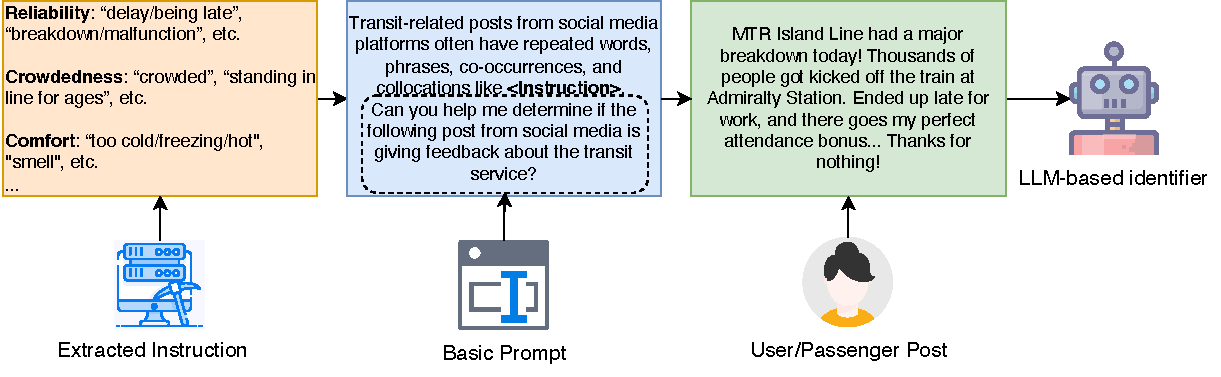
\includegraphics[width=0.95\textwidth]{figs/instru_cept.pdf}
\caption{Instruction-guided filtering of transit feedback}\label{fig:instru_cept}
\end{figure}

To enhance the reliability of the filtering process, two key aspects are integrated: (1) individual optimization of the accuracy of each LLM, and (2) achieving a high level of consensus across the LLMs. The final decision on every post comes from a majority vote, with the minority following the choice taken by the majority. Specifically, for each post \(\boldsymbol{x}_i\), the predicted label is:
\begin{equation}
y_i = \begin{cases} 
1 & \text{if } \sum_{k=1}^{K} \mathbb{I}(p_{k,i} > 0.5) > \frac{K}{2} \\
0 & \text{otherwise}
\end{cases}
\end{equation}
where \(p_{k,i} = P(y_{k,i} = 1 \mid \boldsymbol{x}_i, \boldsymbol{z})\) is the probability output of \(k\) -th LLM for post \(i\), and \(\mathbb{I}(\cdot)\) is the indicator function.

\subsubsection{The filtering problem modeling}

To achieve high accuracy and agreement, we cast the problem as an optimization problem with Kullback-Leibler (KL)-dissimilarity constraint \citep{gultekin2017nonlinear, huang2019novel, liu2024network}. The objective is to find an instruction \(\boldsymbol{z}\), which maximizes the average accuracy of large language models (LLMs), subject to the condition that their output distributions have a cumulative KL divergence within some bounds. More formally, the problem can be formulated as follows.
\begin{equation}
\begin{aligned}
    \underset{\boldsymbol{z}}{\arg\max} \,\, & 
    \frac{1}{K} \sum_{k=1}^{K} \mathbb{E}_{\boldsymbol{y}_{k} \sim \theta_{k}(\boldsymbol{y}_{k} \mid \boldsymbol{X}, \boldsymbol{z})} \left[ a(\boldsymbol{y}_{k}, \boldsymbol{\bar{y}}) \right] \\
    \text{s.t.} \,\, & 
    \sum_{k=1}^{K-1} \sum_{k'=k+1}^{K} \sum_{i=1}^{N} \mathbb{D}_{\text{KL}} \left( \theta_{k}(y_{k,i} \mid \boldsymbol{x}_i, \boldsymbol{z}) \parallel \theta_{k'}(y_{k',i} \mid \boldsymbol{x}_i, \boldsymbol{z}) \right) \leq \epsilon
\end{aligned}
\end{equation}
where:
\begin{itemize}
    \item \(\boldsymbol{\bar{y}} = \{\bar{y}_1, \bar{y}_2, \ldots, \bar{y}_N\}\) is the ground truth labels that indicate whether each post is truly related to transit services.
    \item \(\theta_k(\boldsymbol{y}_k \mid \boldsymbol{X}, \boldsymbol{z})\) is the probability distribution over the labels for all posts, as predicted by the \(k\)-th LLM with instruction \(\boldsymbol{z}\).
    \item \(a(\boldsymbol{y}_{k}, \boldsymbol{\bar{y}})\) is the accuracy of the \(k\)-th LLM's predictions, defined as:
    \begin{equation}
    a(\boldsymbol{y}_{k}, \boldsymbol{\bar{y}}) = \frac{1}{N} \sum_{i=1}^{N} \mathbb{I}(y_{k,i} = \bar{y}_i)
    \end{equation}
    where \(\mathbb{I}(\cdot)\) is the indicator function, returning 1 if the condition is true and 0 otherwise.
    \item \(\mathbb{D}_{\text{KL}} \left( \theta_{k}(y_{k,i} \mid \boldsymbol{x}_i, \boldsymbol{z}) \parallel \theta_{k'}(y_{k',i} \mid \boldsymbol{x}_i, \boldsymbol{z}) \right)\) is the KL divergence between the Bernoulli distributions of the probabilities predicted for post \(i\) by LLMs \(k\) and \(k'\), assuming independence across posts.
    \item \(\epsilon\) is a small positive constant that controls the allowed discrepancy between the LLMs' predictions.
\end{itemize}

The objective function tries to maximize the average accuracy of LLMs, while the constraint that accompany it ensures that the sum of all Kullback-Leibler (KL) divergences between each pair of LLMs across all posts does not exceed \(\epsilon\), thus encouraging agreement among LLMs. The summation over the upper right portion (for \(k=1\) to \(K-1\) and \(k'=k+1\) to \(K\)) avoids revisiting the computations of pairwise KL divergences.

To solve the constrained optimization problem, one derives the Lagrangian dual with a Lagrange multiplier \(\lambda \geq 0\) to impose the KL divergence constraint. The Lagrangian can be written as
\begin{equation}
\begin{aligned}
\mathcal{L}(\boldsymbol{z}, \lambda) &= \frac{1}{K} \sum_{k=1}^{K} \mathbb{E}_{\boldsymbol{y}_{k} \sim \theta_{k}(\boldsymbol{y}_{k} \mid \boldsymbol{X}, \boldsymbol{z})} \left[ a(\boldsymbol{y}_{k}, \boldsymbol{\bar{y}}) \right] \\
&\quad + \lambda \left( \epsilon - \sum_{k=1}^{K-1} \sum_{k'=k+1}^{K} \sum_{i=1}^{N} \mathbb{D}_{\text{KL}} \left( \theta_{k}(y_{k,i} \mid \boldsymbol{x}_i, \boldsymbol{z}) \parallel \theta_{k'}(y_{k',i} \mid \boldsymbol{x}_i, \boldsymbol{z}) \right) \right)
\end{aligned}
\end{equation}
Here, the first term refers to the mean accuracy that is to be achieved with \(K\) LLMs while the latter restricts KL divergence using \(\lambda\) as a parameter to control the trade-off between the increase in accuracy and the consensus among models.

\subsubsection{Instruction refinement for passenger post filtering}

Due to the complexity of analytically finding the best instruction \( \boldsymbol{z}^{*} \), we propose an iterative approach to update the instruction \( \boldsymbol{z}_j \) in each iteration \( j \). Instruction \( \boldsymbol{z}_j \) consists of frequently occurring words, phrases, co-occurrences, and collocations from posts identified as relating to transit services. 

 The iterative instruction refinement process (Algorithm 1) begins with a starting empty instruction \(z_1 = \emptyset\) and an initial prompt, where each of the \(K\) large language models (LLMs) makes predictions about the posts. The first labels \(\boldsymbol{y}_1\) are determined by majority voting among the models. Several features are extracted, such as common occurring unigrams (e.g. "delay"), identified through term frequency; n-grams (e.g., "crowded train"), identified through TF-IDF \citep{qaiser2018text}; co-occurring word pairs (e.g., "late-subway"), rated using pointwise mutual information (PMI) \citep{khan2016sentimi}; and statistically significant collocations (e.g., "broken escalator"), retrieved from transit-related posts \(\boldsymbol{X}_1\). These determined features are used to develop a refined instruction \(z_2\), which is used to improve the prompt for subsequent iterations. In every iteration \(j \geq 2\), the LLMs use the updated prompt to re-evaluate posts, with the majority vote \(\boldsymbol{y}_j\) informing further feature extraction for \(\boldsymbol{z}_{j+1}\). The iterative process continues until the accuracy of the majority vote \(a(\boldsymbol{y}_j, \boldsymbol{\bar{y}})\) stabilizes (i.e. shows changes less than a given threshold \(\delta\)) or passes a target threshold (e.g., 0.9). At this point, the best instruction \(\boldsymbol{z}^*\) and the filtered posts \(\boldsymbol{X}'\) are produced as outputs. The iterative refinement ensures that the instruction increasingly incorporates linguistic patterns, thus improving the LLMs' ability to distinguish authentic transit feedback from spurious references. The pseudo-code describing the instruction refinement is shown in \hyperref[alg:alg1]{Algorithm.\ref{alg:alg1}}.

\begin{algorithm}
\caption{Iterative Instruction Refinement for LLM-based Filtering}
\label{alg:alg1}
\KwIn{Social media posts $\boldsymbol{X} = \{\boldsymbol{x}_1, \ldots, \boldsymbol{x}_N\}$; Number of LLMs $K$ (odd); Ground truth labels $\boldsymbol{\bar{y}}$; Convergence threshold $\delta$; Max iterations $J$}
\KwOut{Identified transit-related posts $\boldsymbol{X}'$; Optimal instruction $\boldsymbol{z}^*$}
Initialize $j \leftarrow 1$, $\boldsymbol{z}_j \leftarrow \emptyset$, prev\_acc $\leftarrow 0$, converged $\leftarrow$ False\;

\While{$j \leq J$ \textbf{and} \textbf{not} converged}{
    \For{$k = 1$ \textbf{to} $K$}{
        $\boldsymbol{y}_{k,j} \leftarrow \theta_k(\boldsymbol{X}|\boldsymbol{z}_j)$ \tcp*{LLM predictions}
    }
    
    $\boldsymbol{y}_j \leftarrow \text{MajorityVote}(\{\boldsymbol{y}_{1,j}, \ldots, \boldsymbol{y}_{K,j}\})$\;
    curr\_acc $\leftarrow \frac{1}{N}\sum_{i=1}^N \mathbb{I}(y_{j,i} = \bar{y}_i)$ \tcp*{Calculate accuracy}
    
    \eIf{$|\text{curr\_acc} - \text{prev\_acc}| < \delta$ \textbf{or} curr\_acc $\geq 0.9$}{
        converged $\leftarrow$ True\;
    }{
        $\boldsymbol{X}' \leftarrow \{\boldsymbol{x}_i \in \boldsymbol{X} | y_{j,i} = 1\}$ \tcp*{transit-related post samples}
        $\boldsymbol{z}_{j+1} \leftarrow \text{ComposePrompt}(\text{ExtractFeatures}(\boldsymbol{X}'))$\;
        $j \leftarrow j + 1$\;
        prev\_acc $\leftarrow$ curr\_acc\;
    }
}

$\boldsymbol{X}' \leftarrow \{\boldsymbol{x}_i \in \boldsymbol{X} | y_{j,i} = 1\}$\;
$\boldsymbol{z}^* \leftarrow \boldsymbol{z}_j$\;

\Return $\boldsymbol{X}', \boldsymbol{z}^*$\;
\end{algorithm}

\subsection{Spatio-temporal information embedding for transit satisfaction evaluation}\label{sec:SatisfMethod}
After applying the instruction-guided filtering model described in Section~\ref{sec:filtering}, which produces a refined collection of transit-related social media posts represented as $\boldsymbol{X}'$, the next objective is the accurate evaluation of passenger satisfaction reflected in this data collection. Section~\ref{sec:filtering} focused on ensuring that the analyzed posts genuinely reflect passenger experiences by minimizing false positives. Here, this section describes the task of correctly determining the sentiment conveyed in these real posts. Observing that conventional sentiment analysis models overlook important spatial and temporal contexts inherent in transit feedback (e.g., the specific location of a transit station or the time of day a comment is made), which can influence passenger attitudes, we present a spatio-temporal tuning mechanism to improve the assessment in the TranSenti model. To fill this gap, we integrate spatio-temporal embeddings into a pre-trained RoBERTa model to facilitate a more accurate and contextualized assessment of passenger satisfaction from filtered social media posts ($\boldsymbol{X}'$).

\subsubsection{Semantic learning of passenger feedback}

Our approach uses the RoBERTa model, which is found to be effective in capturing complex contextual representations of text information \citep{liu2019roberta}. For every post on social networks that is relevant to transit (i.e., filtered entry \(i\) \(X_i\) \(X'\)), RoBERTa takes input and produces a sequence of hidden states of the final layer \(h_i = [h_1,h_2,\ldots,h_s]\) \(R^{s \times d}\), with \(s\) being the sequence length and \(d\) being the dimension of the hidden state (e.g., 768 for RoBERTa base). We obtain three different representations from these hidden states to represent different aspects of content text:

\begin{itemize}
    \item \textbf{Pooler Output (\(\boldsymbol{h}_p\))}: It is calculated using the initial state's hidden state (also called \texttt{[CLS]} token and represented by \(\boldsymbol{h}_0\)), applying to it a linear transformation followed by a tanh activation function:
    \begin{equation}
            \boldsymbol{h}_p = \tanh(\boldsymbol{W}_{\text{pool}} \boldsymbol{h}_0 + \boldsymbol{b}_{\text{pool}}) \in \mathbb{R}^{d}
    \end{equation}
    where \(\boldsymbol{W}_{\text{pool}} \in \mathbb{R}^{d \times d}\) and \(\boldsymbol{b}_{\text{pool}} \in \mathbb{R}^{d}\) are trainable parameters. This representation encapsulates the overall semantic meaning of the input sequence.
    \item \textbf{Average Pooling (\(\boldsymbol{h}_{\text{avg}}\))}: This is the mean of all hidden states across the sequence:
    \begin{equation}
        \boldsymbol{h}_{\text{avg}} = \frac{1}{S} \sum_{j=1}^{S} \boldsymbol{h}_j \in \mathbb{R}^{d}
    \end{equation}
    Average pooling aggregates information from all tokens, providing a general context of the post.
    \item \textbf{Max Pooling (\(\boldsymbol{h}_{\text{max}}\))}: This is the element-wise maximum across all hidden states in the sequence:
    \begin{equation}
        \boldsymbol{h}_{\text{max}} = \max_{j=1}^{S} \boldsymbol{h}_j \in \mathbb{R}^{d}
    \end{equation}
    Max pooling highlights the most salient features, emphasizing key phrases or words that strongly influence sentiment.
\end{itemize}

These three representations are concatenated to form a comprehensive text representation:
\begin{equation}
\boldsymbol{h}_{\text{text}} = [\boldsymbol{h}_p; \boldsymbol{h}_{\text{avg}}; \boldsymbol{h}_{\text{max}}] \in \mathbb{R}^{3d}
\end{equation}
This multi-faceted approach ensures that the model captures both global semantics and local textual features of passenger feedback, enhancing its ability to discern nuanced sentiments in transit-related posts.

\subsubsection{Spatio-temporal feature extraction}
Accurate extraction of spatio-temporal features forms the foundation for reliable transit satisfaction analysis. While for each microblog post $\boldsymbol{x}_i$ the timestamp $t_i$ can be directly extracted from the post itself, we develop a multi-stage geoparsing framework with topological constraints to extract the spatial information from the poststhrough the following key steps.

The first stage involves candidate generation using a bi-directional LSTM-CRF model that identifies geographical entities, pre-trained on the custom transit corpus containing station aliases and landmark associations. This model leverages the sequential nature of text to capture contextual information that helps distinguish geographical references from other named entities. The second step implements topology-aware resolution that maps candidates to the metro network $G=(V,E)$, such as the one shown in \hyperref[fig:SZ_network]{Fig.\,\ref{fig:SZ_network}}, through confidence scoring. The confidence score for each candidate location $v$ is calculated as
\begin{equation}
c(v) = \alpha \cdot f_{\text{edit}}(v,\boldsymbol{x}_i) + \beta \cdot f_{\text{co-occur}}(v,\boldsymbol{x}_i) + \gamma \cdot f_{\text{reachability}}(v,G)
\end{equation}
where the parameters $(\alpha,\beta,\gamma)=(0.4,0.3,0.3)$ are determined via grid search, prioritizing topologically reachable stations with lexical proximity. This scoring mechanism combines edit distance similarity, co-occurrence patterns, and network reachability to ensure that extracted locations are both linguistically plausible and topologically valid within the transit network. The final step performs hierarchical encoding of the confirmed station $v_j \in V$ into multi-dimensional features. Each location is encoded as:
\begin{equation}
l_i = [\text{station ID}, \text{metro line ID}, \text{node ID in}~G]
\end{equation}

\begin{figure}[htbp]
\centering
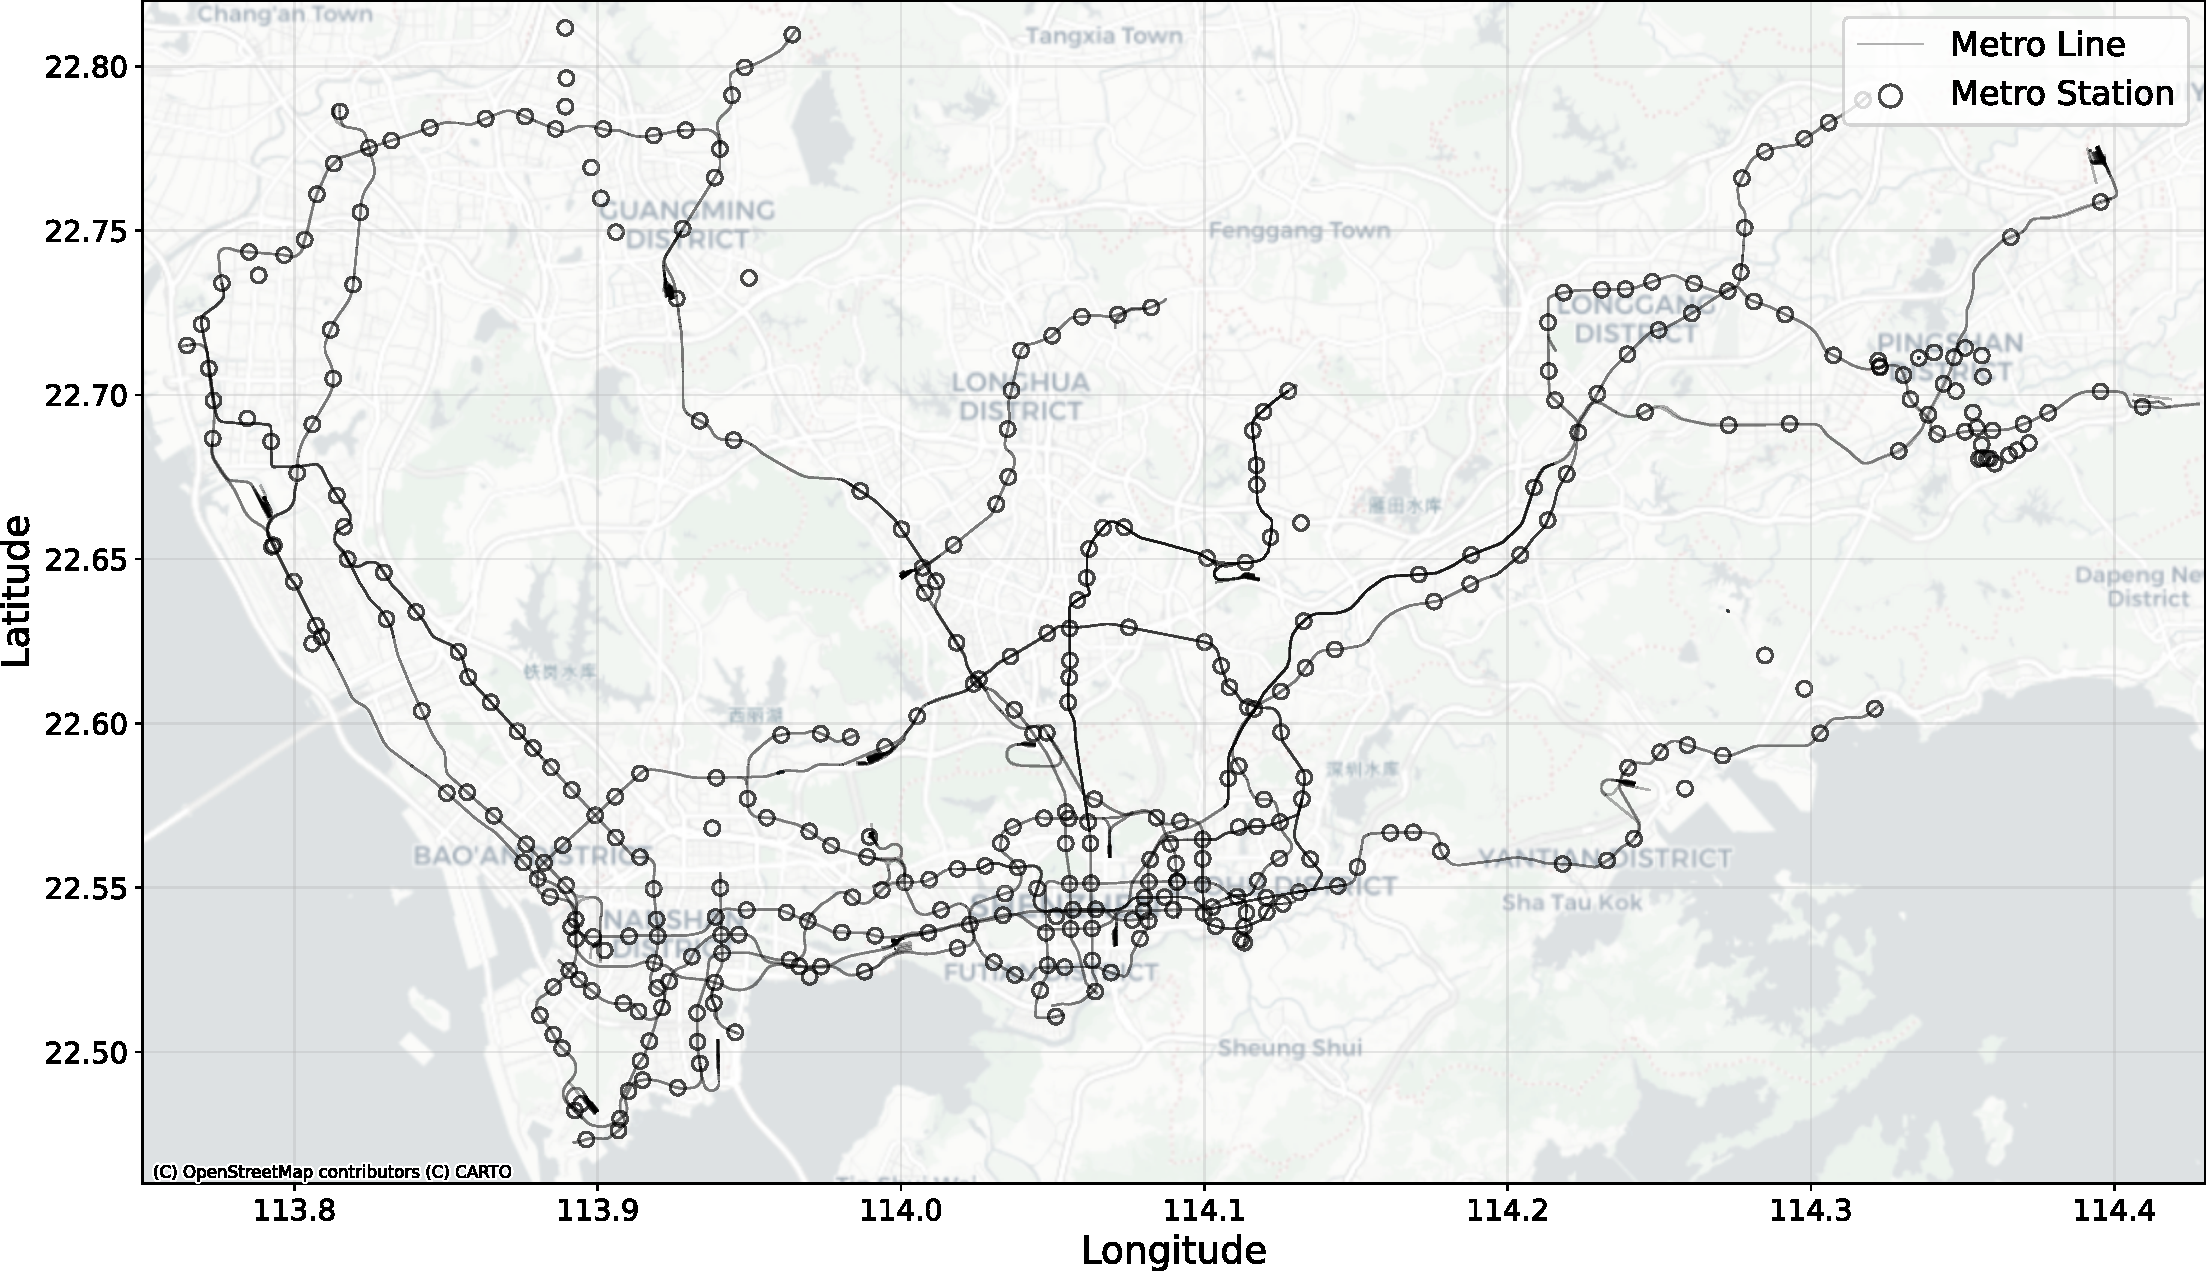
\includegraphics[width=0.8\textwidth]{figs/shenzhen_metro_map.pdf}
\caption{The metro network of Shenzhen}\label{fig:SZ_network}
\end{figure} 

\subsubsection{Spatio-temporal tuning}


To incorporate the spatio-temporal patterns inherent in transit-related posts, we propose a spatio-temporal encoder to examine time \(t_i\) and place \(l_i\) that correspond to every input post \(\boldsymbol{x}_i\). The additional spatio-temporal input helps in effectively grounding sentiment, since passenger experiences vary considerably according to when and where the feedback is posted.
\begin{itemize}
    \item \textbf{Temporal Encoder}:The temporal context \(t_i\) (e.g., the time of the post) is divided into temporal segments, e.g., hourly intervals, based on observed transit operations patterns. An embedding layer maps each temporal segment to a vector representation:
    \begin{equation}
        \boldsymbol{e}_{t_i} = \boldsymbol{E}_t \cdot \text{one\_hot}(t_i) \in \mathbb{R}^{d_t}
    \end{equation}
    where \(\boldsymbol{E}_t \in \mathbb{R}^{T \times d_t}\) is a parameterized temporal embedding matrix with \(T\) being the number of time segments and \(d_t\) being dimension of temporal embedding (e.g., 64). Such encoding can represent temporal contexts, such as peak hours or off-hour patterns, which have a considerable impact on passenger experiences.

    \item \textbf{Spatial Encoder}: The geographical coordinate \(l_i\), referring to a station or stop determined through geo-parsing of \(\boldsymbol{x}_i\), is converted to an embedding vector:
    \begin{equation}
        \boldsymbol{e}_{l_i} = \boldsymbol{E}_l \cdot \text{one\_hot}(l_i) \in \mathbb{R}^{d_l}
    \end{equation}
    where \(\boldsymbol{E}_l \in \mathbb{R}^{L \times d_l}\) refers to spatial embedding matrix with \(L\) being the number of distinct locations and \(d_l\) being spatial embedding dimension (e.g., 64). The embeddings allow the model to learn to capture attributes related to particular locations, such as the congestion level or the state of the infrastructure, thus implicitly capturing the topology of the network described as \(G = (V, E)\).
\end{itemize}
The combination of spatio-temporal embeddings with text representations gives rise to a single input that is then sent to the classification head:
\begin{equation}
    \boldsymbol{h}_{\text{combined}} = [\boldsymbol{h}_{\text{text}}; \boldsymbol{e}_{t_i}; \boldsymbol{e}_{l_i}] \in \mathbb{R}^{3d + d_t + d_l}
\end{equation}
This integration allows us to evaluate text sentiment together with spatio-temporal context to provide more complete passenger sentiment understanding, thus offering a more accurate evaluation of transit service through passenger satisfaction.

The final part is an estimation layer that calculates \( \boldsymbol{h}_{\text{combined}} \) to produce sentiment scores related to both positive and negative satisfaction. Considering the requirement to handle both sentiments individually (as explained in Section \ref{sec:preliminaries}), a linear layer is applied, followed by a sigmoid activation function:
\begin{equation}
    (s^{(i)}_{p}, s^{(i)}_{n}) = \sigma(\boldsymbol{W} \boldsymbol{h}_{\text{combined}} + \boldsymbol{b})
\end{equation}
where \(\boldsymbol{W} \in \mathbb{R}^{2 \times (3d + d_t + d_l)}\) and \(\boldsymbol{b} \in \mathbb{R}^{2}\) are learnable parameters, \(\sigma\) is the sigmoid function, and \(s^{(i)}_{p}, s^{(i)}_{n} \in [0,1]\) represent positive and negative sentiment scores, respectively. The flow chart of the proposed spatio-temporal tuned RoBERTa model is illustrated in \hyperref[fig:spatiotemporal_RoBERTa]{Fig.\,\ref{fig:spatiotemporal_RoBERTa}}.

\begin{figure}[htbp]
\centering
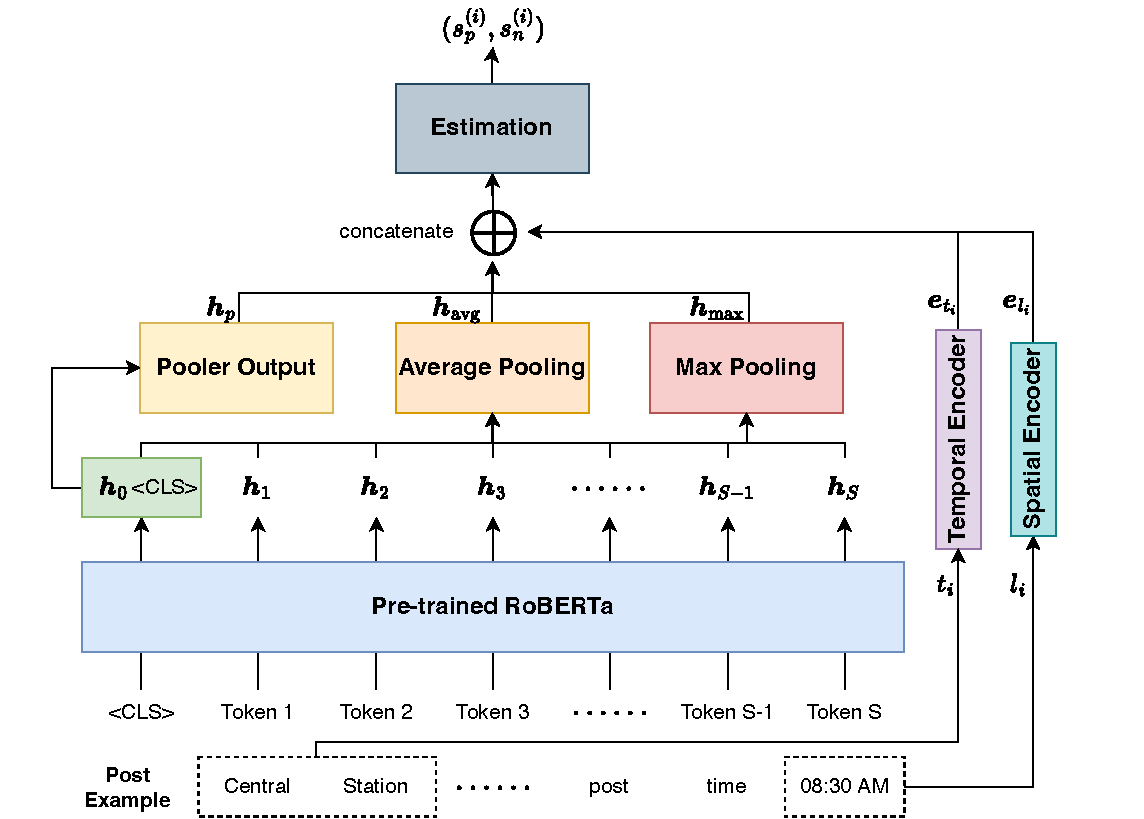
\includegraphics[width=0.9\textwidth]{figs/spatiotemporal_RoBERTa.pdf}
\caption{An illustration of the RoBERTa model with spatio-temporal tuning }\label{fig:spatiotemporal_RoBERTa}
\end{figure}

To specialize the model for the transit satisfaction evaluation, we fine-tune the entire architecture, including the pre-trained RoBERTa parameters, the spatio-temporal embedding layers, and the classification head, on a labeled dataset of social media posts related to transit. Each post in the data set is annotated with ground-truth sentiment labels corresponding to positive and negative feedback, enabling supervised learning. The objective of the training process is to minimize the binary cross-entropy loss for each sentiment label:
\begin{equation}
    \textit{Loss} = -\frac{1}{N} \sum_{i=1}^{N} \left[ \bar{s}^{(i)}_{p} \log(s^{(i)}_{p}) + (1 - \bar{s}^{(i)}_{p}) \log(1 - s^{(i)}_{p}) + \bar{s}^{(i)}_{n} \log(s^{(i)}_{n}) + (1 - \bar{s}^{(i)}_{n}) \log(1 - s^{(i)}_{n}) \right]
\end{equation}

Here, \( \bar{s}^{(i)}_{p} \) and \( \bar{s}^{(i)}_{n} \) refer to actual tags corresponding to positive and negative sentiments, respectively, while \( N \) is the number of posts in the training set. By using this fine-tuning technique, the model learns to analyze textual features with spatio-temporal features like co-occurring crowding complaints and peak hours in heavily used stations.

In an effort to avoid overfitting while allowing RoBERTa to take advantage of the rich reservoir of information inherent in its design, we use differential learning rates. In particular, a lower learning rate (for example, \(2 \times 10^{-5}\)) is used for the existing parameters pre-trained by RoBERTa, while a higher learning rate (for example, \(1 \times 10^{-3}\)) is used for the newly introduced spatiotemporal encoders and classification head. This practice aims to create a balance between adapting to the transit environment and maintaining RoBERTa's linguistic competency in general sentiment analysis. By including spatio-temporal encoding, this offers several benefits over traditional sentiment models. By explicitly encoding time context (e.g., peak hours of operation) and space context (e.g., station conditions), the model can identify between sentiments that represent system-wide transit challenges and those that represent short-lived abnormalities. Increasing context awareness not only improves the accuracy of the model, but also increases interpretability, allowing transit agencies to identify operational interruptions with higher accuracy and expanding the applicability of the TranSenti framework to evaluate real-world transit systems.

\section{Case study}\label{sec:experiments}

\subsection{Data collection and preprocessing}

\textbf{Dataset and preprocessing} \quad 
The dataset used in this study consists of Sina Weibo posts that represent a major Chinese social media platform similar to Twitter and are widely used to share updated news. Data were collected by choosing posts containing keywords "metro/subway," while also limiting the spatial scope to Shenzhen, a major city with a highly developed metro system. Through this method, we obtained a set of 512,738 Sina Weibo posts created between January 2019 and January 2022. The posts represent a broad set of viewpoints for passengers, thus offering a comprehensive evaluation of the satisfaction with the Shenzhen metro for the given time interval.

In TranSenti, a chain of pre-processing operations was inserted to condition the data for future analysis. First, the raw text was preprocessed to filter out irrelevant material such as URLs, mentions (@username, for example), hashtags, and non-Chinese characters that are not related to the transit satisfaction examination. The preprocessed text was then processed using tokenization with the Qwen2.5 tokenizer, which is a state-of-the-art tool for Chinese text segmentation that enables post-segmentation of individual words or tokens. In addition, traditional Chinese characters were converted to simplified characters to improve homogeneity in the dataset. To help with model evaluation, a random sample of 4,500 posts was obtained and labeled by hand by two domain experts with a 95\% inter-annotator agreement rate. Discrepancies that emerged were addressed through discussion to arrive at fine-tuning and test sets that included ground-truth tags for filtration and satisfaction classification assessment.

\subsection{Experiment settings}
\subsubsection{Implementation details}
The TranSenti framework is created by combining LLMs with spatio-temporal context. A mixture-of-experts architecture is used for each stage of hybrid filtering based on four different LLMs: Qwen2.5, Gemini-2.0, DeepSeek-R1, and o3 mini. Each of the models is individually queried in a zero-shot mode to evaluate each social media post to determine individual relevance to transit services. Individual judgments are then combined through a majority vote mechanism (i.e., mixed w/o instruction refers to majority vote without instruction refinement).

For sentiment analysis, a pre-trained RoBERTa-base (125M parameters) spatio-temporal encoding is fine-tuned using 3,500 out of 4,500 mannually labeled samples. Temporal features are obtained by segmenting the timestamps of posts into hourly segments and representing them as vectors of size \(d_t=64\). To derive spatial features, a geoparser is used to decode transit stop names (such as “Shenzhen North Station”), map them onto the metro topology graph \(G=(V,E)\), and represent them as vectors of dimension \(d_l=64\). Experimental validation on Shenzhen Metro data shows 87.6\% parsing accuracy for ambiguous location references (e.g., "the metro station near Science Museum"), outperforming regular expression baselines by 41.2 percentage points. Text embeddings are obtained through RoBERTa by combining pooler output with average pooling and max pooling methods to produce a vector of size 2304. Then, these representations are concatenated with spatial and temporal embeddings to arrive at a final input size of (\(3\times768+64+64=2432\)). Fine-tuning is performed using a binary cross-entropy loss function and differential learning rates: learning rates for pre-trained RoBERTa parameters are set lower (\(2\times10^{-5}\)), while higher (\(1\times10^{-3}\)) learning rate is used for spatio-temporal encoders and classification head. Training is completed using the AdamW optimizer to a maximum of 10 epochs with a batch size of 16 and early stopping practices, to optimize the model with a manually labeled subset of 4,500 posts with training and testing splits to 90\% and 10\%, respectively. 

\subsubsection{Baselines and evaluation metrics} 
To test the effectiveness of TranSenti, we compared it with several powerful baseline methods. These baseline methods for the filtering of social media posts include: Keyword-based filtering (Use a list of keywords such as "subway","metro" and "bus" to find traffic-related posts, but this simple method often catches irrelevant posts that casually mention these words);LLM-based zero-shot filter (Use separate large models such as Qwen2.5, Gemini-2.0, DeepSeek-R1 and o3 mini with common prompt words to identify traffic-related posts); and there is also a mixture-of-experts majority voting baseline (which summarizes the results of these four LLMs by voting, but does not have a section for iterative optimization instructions). Finally, we compared the proposed method that combines mixture-of-experts and instruction refinement with these baseline models, and proved that using an instruction-based mechanism to identify transit-related posts is indeed more advantageous.

In the satisfaction analysis, baseline models refer to those models originally designed for general sentiment analysis and are not specifically optimized for spatio-temporal information in the transportation field. These models include: BERTweet, an LLM optimized for Twitter, uses masked language modeling \citep{nguyen2020bertweet}; TweetNLP, a RoBERTa-based model that specializes in analyzing tweets emotions \citep{camacho2022tweetnlp}; DeepSeek-R1, an LLM that uses reinforcement learning to optimize emotion classification and reasoning models \citep{guo2025deepseek}; Bi-LSTM, a sequential model that understands context and is used to classify emotions \citep{mahadevaswamy2023sentiment}; RoBERTa Base, a RoBERTa model fine-tuned on Twitter datasets for general sentiment analysis \citep{liu2019roberta}; RoBERTa tuned, a fine-tuned version of the RoBERTa base model on tagged traffic posts, and fastText, a lightweight classifier based on character n-grams that quickly classifies text \citep{joulin2017bag}.

Performance is evaluated using a test dataset that is manually annotated with ground-truth labels for the filtering task (transit-related versus non-service) and sentiment task (positive versus negative satisfaction/sentiment). Performance metrics used include accuracy, precision, recall, and F1-score. In the filtering task, accuracy indicates the general correctness of the model, while precision and recall measure the model's ability to correctly identify genuine transit-related posts and avoid false positives. For the sentiment classification task, the metrics measure the performance in differentiating between positive and negative sentiments.

% \subsection{Overall Performance}

% To comprehensively evaluate the effectiveness of our proposed TranSenti framework, this subsection presents an integrated performance analysis that combines both the data filtering and the sentiment classification steps.

% \subsubsection{End-to-end pipeline performance}
% We compared the TranSenti framework with the most recent sentiment analysis method. These comparison methods include: Keyword-based filtering plus universal sentiment models (Keyword + BERTweet, Keyword + TweetNLP, Keyword + RoBERTa Base), separate LLM filtering plus sentiment classifiers (Qwen2.5 + BERTweet, Qwen2.5 + TweetNLP, Qwen2.5 + RoBERTa Base), and our own mixed expert methods without instruction optimization, paired with fine-tuned RoBERTa (Mixture w/o Inst. + RoBERTa Base).

% As illustrated in \hyperref[fig:overall_performance]{Fig.~\ref{fig:overall_performance}}, the  TranSenti framework performs exceptionally well on all test metrics. Its end-to-end F1 score (which is the geometric average of the filtering and sentiment classification F1 scores to consider the coordination of the entire process) is much higher than those baseline combinations. TranSenti's end-to-end F1 score reached 78.9\%, which is 17.8 to 29.8 percentage points higher than those baseline combinations using keyword, and 6.7 to 8.7 percentage points higher than the individual LLM method.

% \begin{figure}[htbp]
% \centering
% 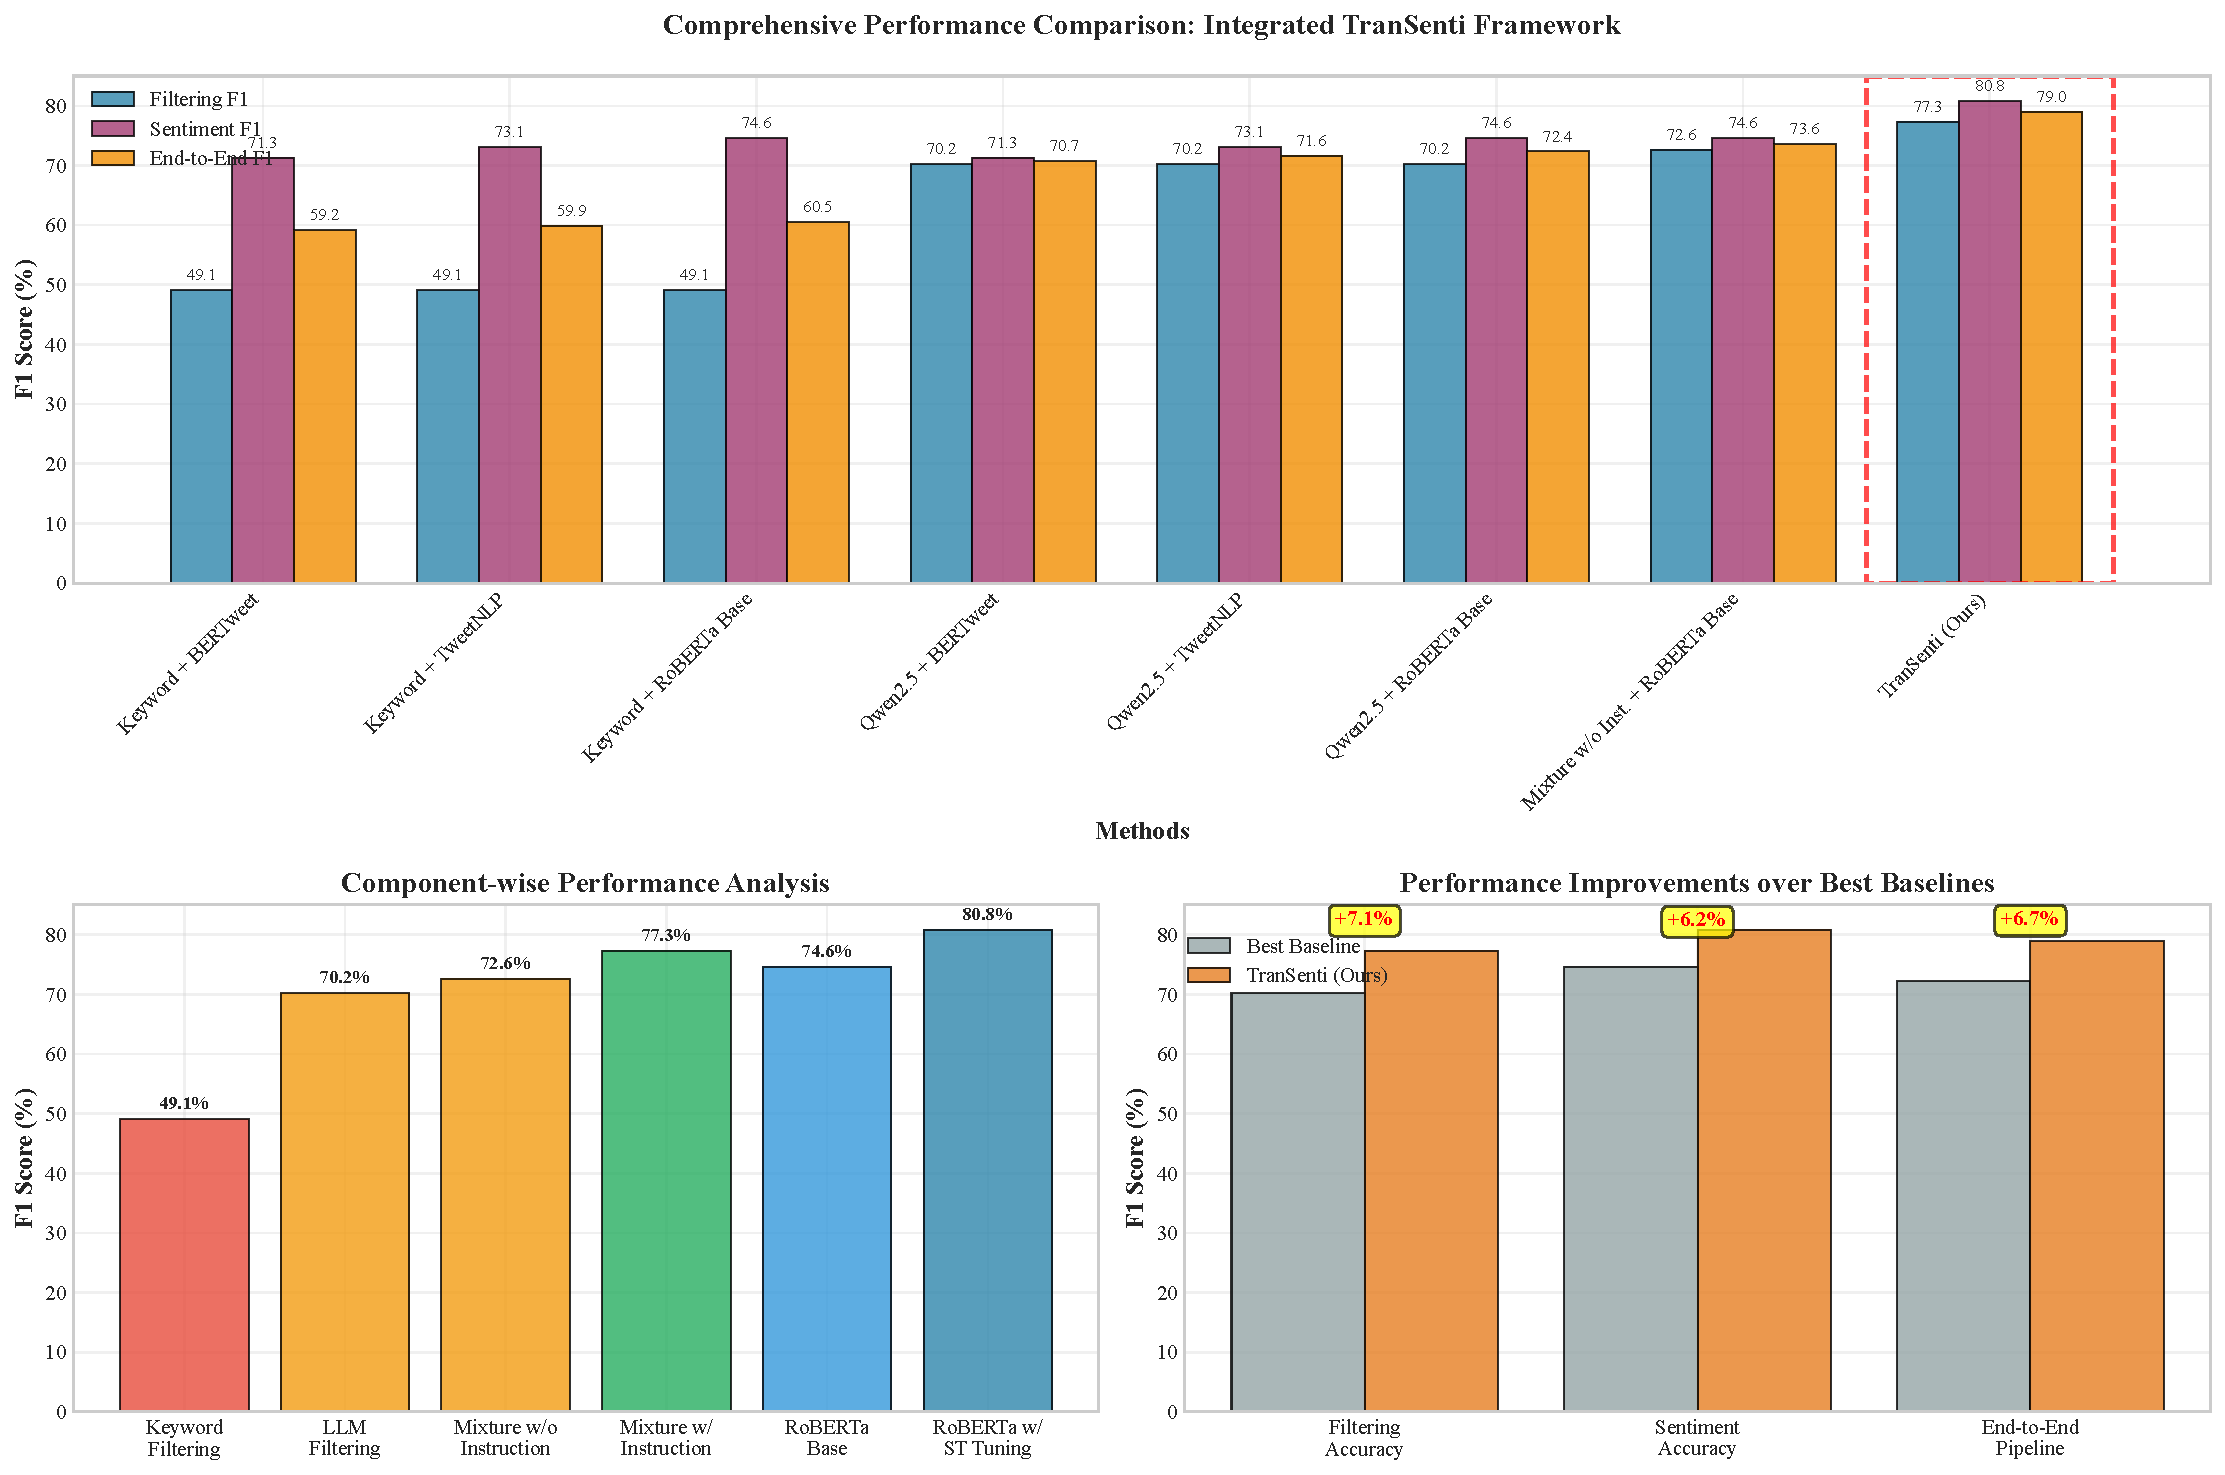
\includegraphics[width=0.99\textwidth]{figs/overall_performance_comparison.pdf}
% \caption{Comprehensive performance comparison of integrated TranSenti framework against state-of-the-art baseline combinations}\label{fig:overall_performance}
% \end{figure}

% Performance analysis showed us several important findings. First, keyword filtering will be stuck. Even if you use the powerful sentiment analysis tool RoBERTa Base, the best keyword combination (Keyword + RoBERTa Base) can only get an F1 score of 61.1\%. Second, a single LLM filter can make the effect better, but because there is no mechanism for everyone to vote together and there is no optimization for specific tasks, the effect is still limited. Third, the "mixture-of-experts" method we developed (without instruction refinement) proved that putting multiple tools together is useful and we can get a F1 score of 73.6\%. Finally, the complete TranSenti framework with instruction refinement and spatio-temporal parameter adjustment has the best effect, which shows that the parts we designed are really good together.

% \subsubsection{Component contribution analysis}
% In order to find out how useful each part of the TranSenti framework is, we conducted an ablation analysis and tested the two modules of filtering and sentiment analysis. As shown in \hyperref[fig:ablation_analysis]{Fig.~\ref{fig:ablation_analysis}}, each part can improve the whole system and the effect is superimposed.

% \begin{figure}[htbp]
% \centering
% 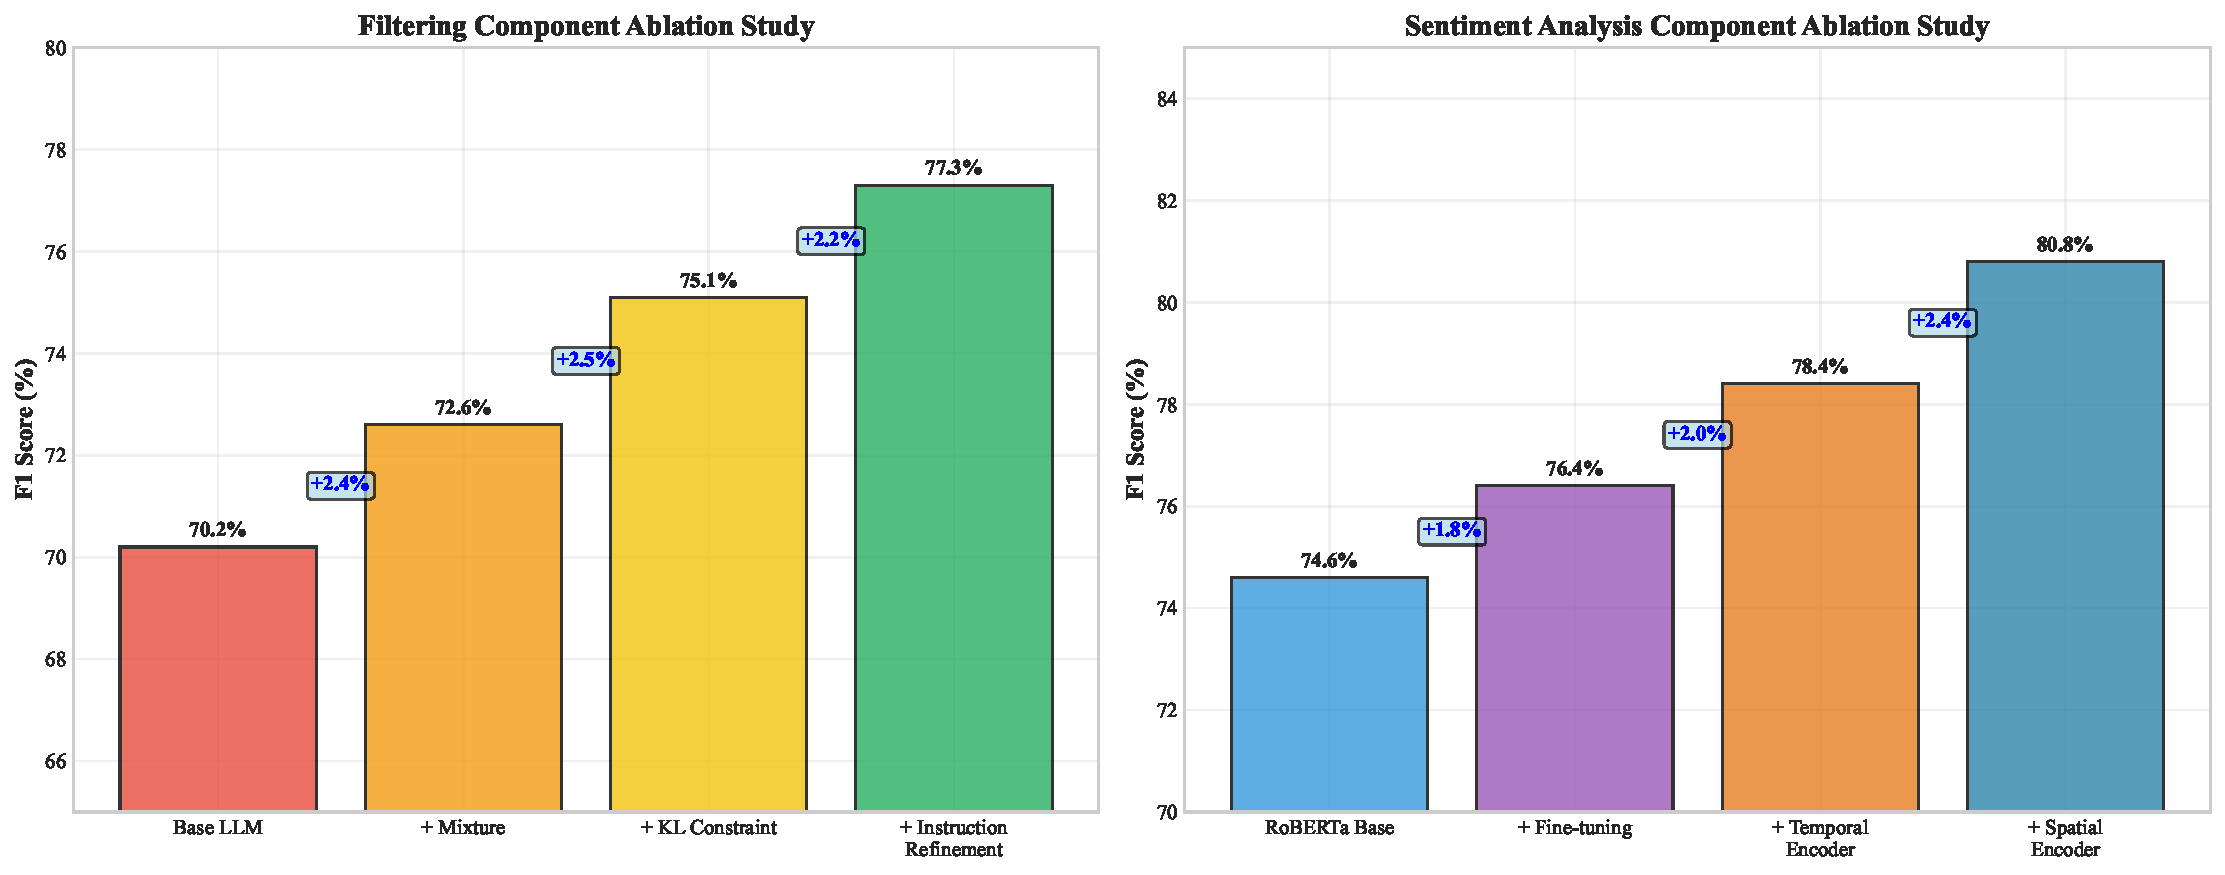
\includegraphics[width=0.99\textwidth]{figs/ablation_study_analysis.pdf}
% \caption{Ablation study analysis showing the contribution of individual components in the TranSenti framework}\label{fig:ablation_analysis}
% \end{figure}

% In the filtering process, the upgrade from base LLM (70.2\% F1) to mixture-of-experts (72.6\% F1) increased by 2.4 percentage points, indicating that multiple experts working together can reduce the number of confusing individual models. After adding the KL-divergence limit, the effect rose to 75.1\% F1 (an increase of 2.5 percentage points), which proves the importance of reaching consensus among models when mixing filtering. The instruction refinement component contributed the largest single improvement (up 2.2 percentage points to 77.3\% F1), validating our iterative domain-specific optimization approach.

% For sentiment analysis, fine-tuning the base RoBERTa model on transit-specific data improves performance from 74.6\% to 76.4\% F1 (1.8 percentage points), establishing the foundation for domain adaptation. The temporal encoder contributes an additional 2.0 percentage points (78.4\% F1), enabling the model to contextualize sentiments based on operational patterns such as peak-hour congestion. The spatial encoder provides the final improvement of 2.4 percentage points (80.8\% F1), allowing the model to associate location-specific feedback with network topology and station characteristics.

% In the following sections, we explore the specifics of the outcomes associated with the two primary stages of our proposed framework.

\subsection{Results of passenger feedback filtering}
This subsection presents our proposed hybrid filtering method to find passenger feedback that is truly related to transit service from social media data. We used a manually annotated dataset to conduct experiments to see how our instruction-guided mixture-of-experts model performed, comparing it with traditional keyword methods and several LLM baselines. 

\subsubsection{Comparison with individual baselines}

To evaluate the effectiveness of our hybrid filtering approach, we compare its performance against keyword-based filtering and individual LLM baselines. \hyperref[tab:filtering_performance]{Table~\ref{tab:filtering_performance}} shows the results on four evaluation metrics: Accuracy, precision, recall, and F1-score. Our proposed method shows improved performance with 78.7\% accuracy and 77.3\% F1-score, reflecting consistent improvements compared to baselines.

\begin{center}
\captionof{table}{Performance comparison of transit-related post filtering methods}
\label{tab:filtering_performance}
\begin{tabular}{lcccc}
\toprule
Method & Accuracy (\%) & Precision (\%) & Recall (\%) & F1-score (\%) \\
\midrule
Keyword-based & 54.5 & 42.3 & 58.7 & 49.2 \\
Qwen2.5 & 68.9 & 65.7 & 72.4 & 68.9 \\
Gemini-2.0 & 64.1 & 60.8 & 68.3 & 64.3 \\
DeepSeek-R1 & 66.7 & 63.5 & 70.6 & 66.9 \\
o3 mini & 60.2 & 57.1 & 65.3 & 60.9 \\
Mixture w/o Instruction & 71.5 & 68.9 & 74.2 & 71.5 \\
\textbf{Mixture w/ Instruction (Ours)} & \textbf{78.7} & \textbf{76.4} & \textbf{79.8} & \textbf{78.1} \\
\bottomrule
\end{tabular}
\end{center}

The keyword-based method performs significantly poorly (49.2\% F1), mainly due to the inability to properly distinguish between context-based uses of transit-related vocab. Stand-alone LLMs perform moderately, with Qwen2.5 having the top stand-alone performance (68.9\% F1), reflecting this model's proficiency in semantically understanding microblogs. A large discrepancy is evident across multiple models: Gemini-2.0 has a comparatively low precision rate (60.8\%), reflecting too much inclusion of unclear cases, while o3 mini's low recall (65.3\%) indicates too-conservative classification. The baseline mixture-of-experts model without instruction refinement illustrates the benefits of ensemble learning, with a 2.6 percentage point improvement of the F1 score over the best-performing single model (71.5\% over 68.9\%). Our complete implementation, based on iterative instruction refinement, outperforms all baseline models, with an F1 score of 78.1\%, precision of 76.4\%, and recall of 79.8\%.

It should be noted that while an F1 score of 77. 3\% may appear modest compared to benchmarks in some well-defined NLP classification tasks (which can exceed 90\%), the task of filtering genuine transit service feedback from noisy social media data presents unique challenges. Unlike standard sentiment analysis on curated datasets, this task requires distinguishing subtle contextual differences between actual passenger experiences and incidental mentions (e.g., metaphorical uses of "subway", discussions about locations near stations without commenting on the service itself). The inherent ambiguity and noise in raw informal microblog text make this filtering significantly harder. Therefore, achieving a 77. 3\% F1 score, which represents a substantial improvement of up to 28.2 percentage points over keyword-based methods and notable gains over individual state-of-the-art LLMs, demonstrates the strong capability of our hybrid instruction-guided approach to navigate this complex and noisy data landscape effectively.

\subsubsection{Effectiveness of instruction refinement}

To further investigate the effectiveness and implications of instruction refinement, we evaluate the development of filtering performance based on instruction length and the number of LLMs (\(K\)). \hyperref[fig:instruction_length]{Fig.~\ref{fig:instruction_length}} demonstrates the relationship between the length of the instruction token (from 50 to 500 tokens) and the classification metrics under different ensemble sizes (\(K=2,3,4\)). Three major trends are found: all measures show steady improvement with increasing instruction length, confirming that longer contextual prompts enhance classification performance. For $K=4$, accuracy increases from 71. 5\% with 50 tokens to 78.7\% with 500 tokens (an increase of 7. 2\%), the precision increases from 68. 9\% to 76. 4\%, and recall improves from 74. 2\% to 79. 8\%, indicating an improved balance between reducing false positives and maintaining sensitivity. The size of the ensemble ($K$) significantly impacts the scaling of performance, with 500 token instructions showing that increasing $K$ from 2 to 4 increases the F1 score by 4.4 percentage points (72.9\%$\rightarrow$77.3\%); larger ensembles particularly benefit from the recall: the 4-LLM configuration achieves a recall of 79. 8\% versus 76. 1\% for $K=2$, demonstrating improved coverage of genuine transit posts. The sensitivity of the metrics varies by the granularity of the instruction, with precision exhibiting the steepest gains ($\Delta$ 7.5\% for $K=4$), suggesting detailed instructions help reject borderline cases; recall improvements decelerate beyond 300 tokens, implying diminishing returns in post coverage, with the optimal balance occurring at 500 tokens where all metrics peak without overfitting.

\begin{figure}[!ht]
\centering
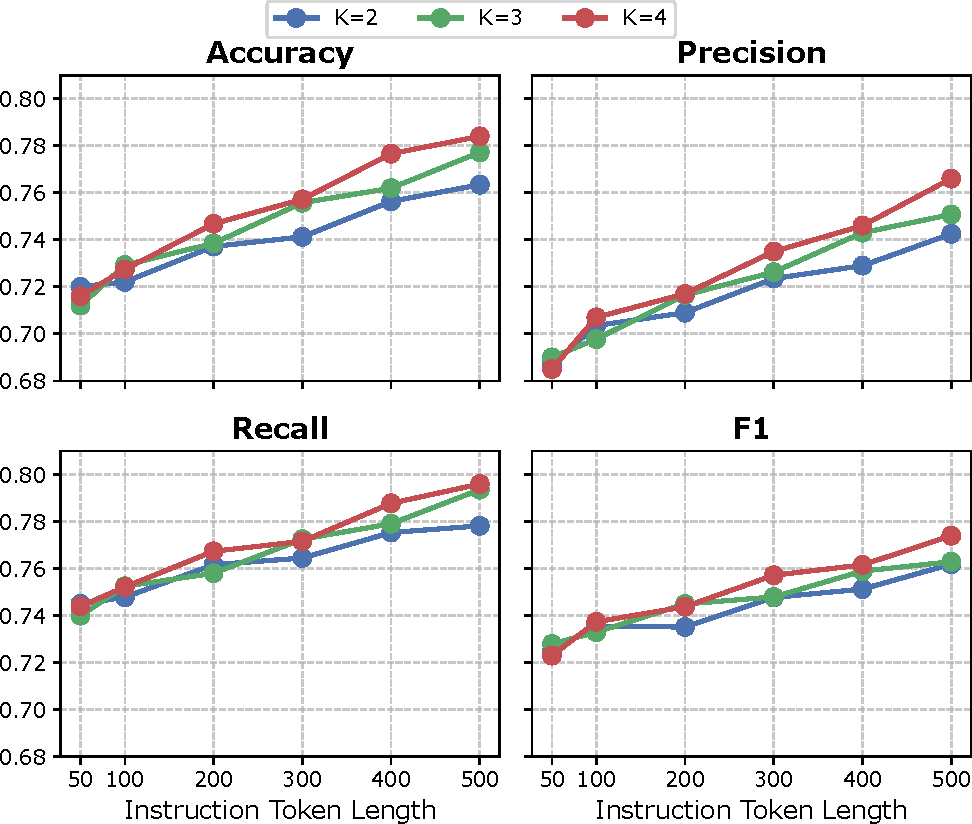
\includegraphics[width=0.55\textwidth]{figs/instruction_length_performance.pdf}
\caption{Performance variation with instruction token length and LLM ensemble size (\(K\))}\label{fig:instruction_length}
\end{figure}

% \subsubsection{Analysis of filtered transit-related content}
% To better understand the characteristics of these selected transport-related posts, we analyzed the thematic content distribution of successfully identified passenger feedback.\ hyperref[fig:wordcloud]{Fig.~\ ref{fig:wordcloud}} shows a word cloud map showing the most frequently mentioned topics and keywords in the filtered dataset, classified according to different service dimensions.

% \begin{figure}[!ht]
% \centering
% 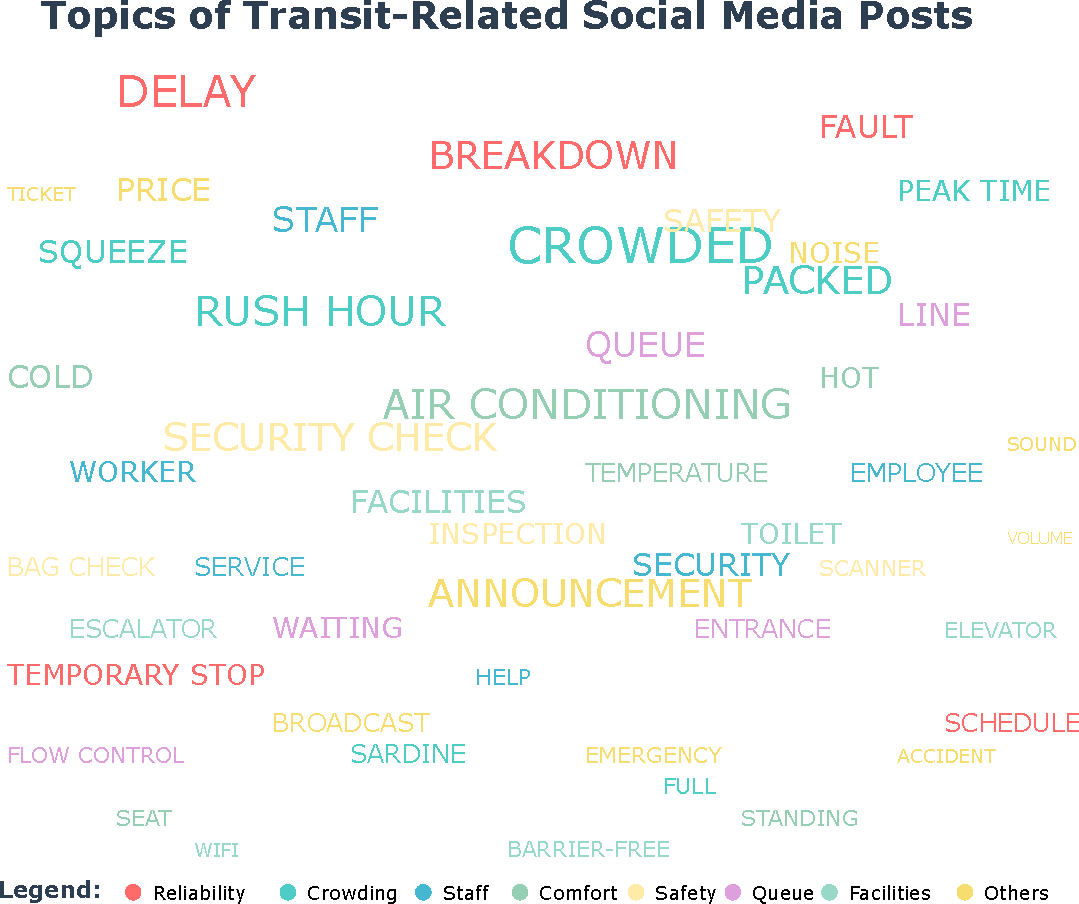
\includegraphics[width=0.75\textwidth]{figs/wordcloud.pdf}
% \caption{Word cloud of topics in filtered transit-related social media posts}\label{fig:wordcloud}
% \end{figure}

% The analysis found that the words related to congestion (marked in bluish green) were the most prominent in the filtered content, with "CROWDED" being the most noticeable keyword, followed by "RUSH HOUR" and "PACKED.", suggesting that passengers' experiences of overcrowding account for a large part of transit-related discussions on the  social media platform. Reliability issues (marked in red) are also prominent, with words like "DELAY","BREAKDOWN" and "FAULT" appearing frequently, reflecting passengers' concerns about service reliability.

% Comments on comfort (green section) mainly mentioned the words like "AIR CONDITIONING", explaining that temperature comfort is a key factor in the passenger experience. Among safety-related topics (yellow part), words such as "SECURITY CHECK","SAFETY" and "INSPECTION" appear, indicating that security measures are also important for the quality of public transport services. The queuing problem (purple part) is reflected through the keywords, such as "QUEUE","LINE" and "WAITING", reflecting the challenges faced by bus operations during peak hours.

\subsection{Results of passenger satisfaction analysis}
Based on the dataset we filtered out, we then use our fine-tuned RoBERTa model to classify the sentiments of passengers' social media posts.
\subsubsection{Comparison with generic sentiment baselines}

As shown in \hyperref[tab:sentiment_comparison]{Table~\ref{tab:sentiment_comparison}}, the optimized spatio-temporal model records an F1 score of 80. 8\%, outperforming all standard sentiment baseline models by between 6.2 and 18.7 percentage points. Twitter-specifically optimized models, i.e., BERTweet (71.3\% F1) and TweetNLP (73.1\% F1), show limited flexibility in adapting to transit scenarios, while RoBERTa Base (74.6\% F1) reaffirms the semantic dominance of transformers over more lightweight models such as fastText (62.1\% F1). The performance gap stems from the inability of generic models to precisely interpret context-dependent sentiments, such as the difference between peak-hour congestion and isolated incidents.


\begin{center}
\captionof{table}{Performance comparison of sentiment analysis methods on transit service posts}
\label{tab:sentiment_comparison}  
\begin{tabular}{lcccc}  
\toprule  
Model & Accuracy (\%) & Precision (\%) & Recall (\%) & F1-score (\%) \\
\midrule  
BERTweet & 68.2 & 70.5 & 72.1 & 71.3 \\
TweetNLP  & 69.8 & 72.3 & 73.8 & 73.1 \\
DeepSeek-R1 & 65.4 & 67.9 & 69.2 & 68.5 \\
Bi-LSTM  & 62.1 & 64.7 & 66.3 & 65.5 \\
RoBERTa Base  & 71.6 & 73.8 & 75.4 & 74.6 \\
fastText  & 58.9 & 61.2 & 63.0 & 62.1 \\
\textbf{RoBERTa w/ ST Tuning (Ours)} & \textbf{78.7} & \textbf{80.2} & \textbf{81.5} & \textbf{80.8} \\
\bottomrule  
\end{tabular}  
\end{center}

The proposed model achieves 78.7\% accuracy and 80.2\% precision, reflecting its effectiveness in identifying genuine feedback versus redundant information. This improvement highlights the importance of spatio-temporal optimization: temporal encoding adds context awareness to time-sensitive matters (e.g., delays in off-peak times), whereas spatial features connect grievances to operational habits of particular stations. By comparison, baseline architectures fail to extract sentiments surrounding transit dynamics and continue to misclassify context-based feedback.

\subsubsection{Effectiveness of fine tuning}

In addition to testing the efficacy of spatio-temporal tuning, this work also offers a classification of passenger satisfaction based on different dimensions of service. As seen in \hyperref[fig:roberta_comparison]{Fig.,\ref{fig:roberta_comparison}}, the tuned spatio-temporal RoBERTa outperforms its baseline counterpart (also fine-tuned with labeled passenger posts) with average accuracy gains between 4.8\% and 9.4\% with respect to reliability, crowdedness, and safety. In particular, the detection of negative sentiment on crowdedness experiences improves by 8.4 percentage points (from 71. 7\% F1 score to 80. 1\% F1 score) by enabling differentiation between peak-hour system congestion and random events. In addition, the precision of the positive sentiment in safety-related comments improves by a factor of three (from 16. 7\% F1 score to 50. 0\% F1 score) by linking to infrequent compliments.

\begin{figure}[htbp]
\centering
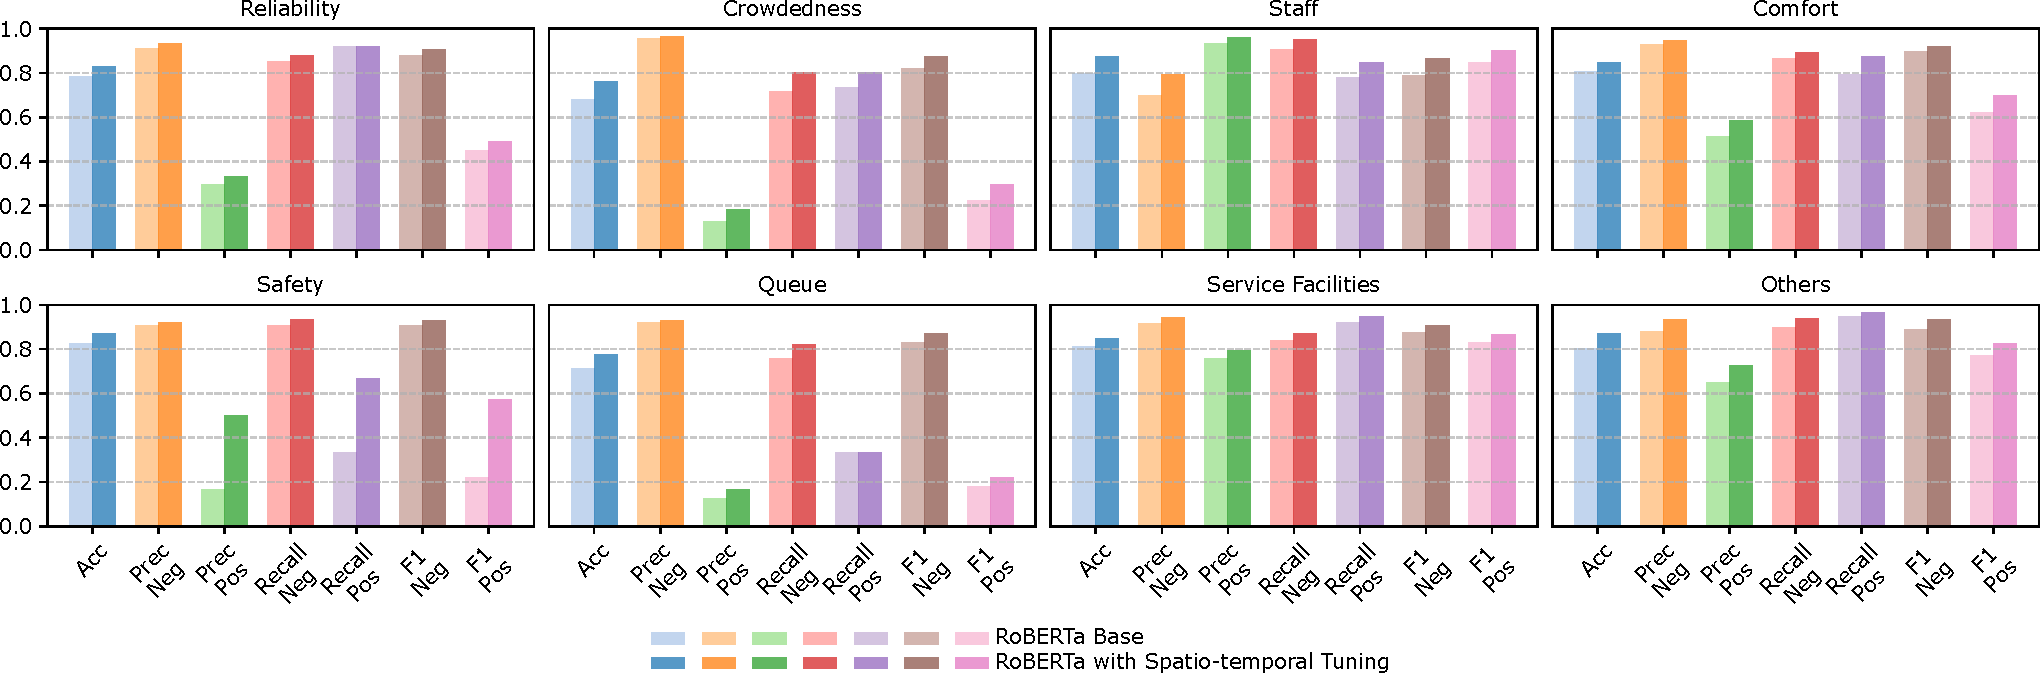
\includegraphics[width=0.99\textwidth]{figs/roberta_comparison_h.pdf}
\caption{Performance Comparison: RoBERTa Tuned vs. RoBERTa with Spatio-temporal Tuning}\label{fig:roberta_comparison}
\end{figure}

The contextualization in the proposed method also reduces the misclassification of transient difficulties to systemic flaws, since it has been shown to improve by 53. 4\% in the contextually relevant positive F1 score (0.901 to 0.848) for staff-related comments. The results are consistent with the idea that explicit spatio-temporal encoding resolves basic shortcomings found in typical sentiment models. By capturing textual feedback in transit contexts, the improved model achieves improvements between 5. 9\% and 12. 3\% on contextually relevant topics such as queue management and service infrastructure.

\subsubsection{Ablation analysis of spatio-temporal modules}

In an attempt to gauge the spatio-temporal effects, we conduct an ablation study that compares settings with and without spatial and/or temporal encoders. The findings presented in \hyperref[fig:ablation]{Fig.~\ref{fig:ablation}} show that in four different evaluation measures; both modules contribute to satisfaction classification, with the temporal context having a greater effect.

The removal of temporal encoding (RoBERTa without Temporal) sees a strong drop in performance, with the F1 score decreasing by 4.9 percentage points (from 80.8\% to 75.9\%). The decreases in precision and recall ($\Delta$4.6\% and $\Delta$5.3\%) reflect the misclassification of time-dependent sentiments; e.g., not associating "delays" with peak-hour congestion trends. Conversely, removing spatial encoding (RoBERTa without Spatial) produces smaller drops (F1 $\Delta$2.4\%), as location-agnostic models still collect complaints that are station independent, e.g., "uncomfortable seats." However, both ablated models outperform the base RoBERTa Tuned model (F1 74. 6\%), demonstrating that even partial context incorporation helps in classification results. The superior performance of the complete model (80.8\% F1) demonstrates the complementary nature of spatio-temporal context learning. 

\begin{figure}[htbp]
\centering
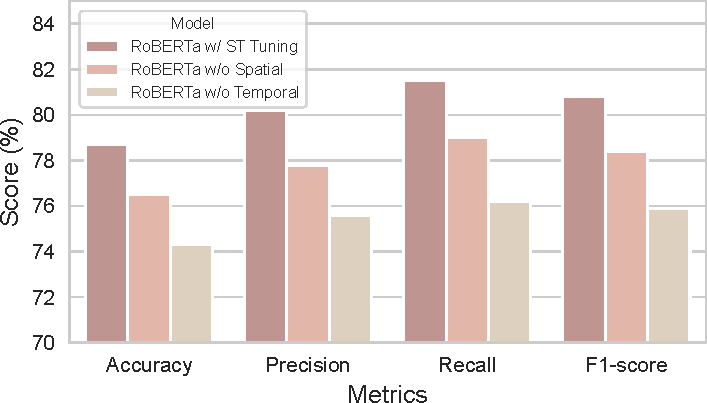
\includegraphics[width=0.65\textwidth]{figs/ablation.pdf}
\caption{Ablation study of spatio-temporal components}\label{fig:ablation}
\end{figure}

% \subsection{Spatio-Temporal Sentiment Distribution Analysis}\label{sec:spatiotemporal}

% TranSenti adds spatio-temporal context, allowing us to comprehensively analyze sentiment distribution patterns from both spatial and temporal dimensions, which provides an important reference for traffic management and service improvement. We plot the distribution of negative and positive sentiments in time and space according to different service dimensions to analyze passenger satisfaction (or dissatisfaction) with transit services.

% \subsubsection{Spatial Distribution Patterns}

% The spatial analysis reveals distinct spatial clustering patterns in passenger sentiment across the Shenzhen Metro network. As shown in \hyperref[fig:comfort_negative]{Fig.~\ref{fig:comfort_negative}} and \hyperref[fig:comfort_positive]{Fig.~\ref{fig:comfort_positive}}, comfort-related sentiments exhibit strong spatial heterogeneity, with negative sentiment concentrations primarily in densely populated urban core areas and major transfer stations. The heatmap illustrating comfort-related negative sentiments highlights significant hotspots within the central areas of both the Futian District and Luohu District, locations where many metro lines intersect and which typically exhibit the high passenger flow. The areas exhibiting the highest positive sentiment are located in the city's peripheral regions, specifically near metro stations such as Lingzhi and Baoan Center.

% \begin{figure}[htbp]
% \centering
% \includegraphics[width=0.9\textwidth]{figs/spatio_distribution_vis/shenzhen_metro_comfort_negative_sentiment_unified_normalized_heatmap.png}
% \caption{Spatial distribution of comfort-related negative sentiment}\label{fig:comfort_negative}
% \end{figure}

% \begin{figure}[htbp]
% \centering
% \includegraphics[width=0.9\textwidth]{figs/spatio_distribution_vis/shenzhen_metro_comfort_positive_sentiment_unified_normalized_heatmap.png}
% \caption{Spatial distribution of comfort-related positive sentiment}\label{fig:comfort_positive}
% \end{figure}

% Crowdedness sentiment patterns (\hyperref[fig:crowdedness_negative]{Fig.~\ref{fig:crowdedness_negative}} and \hyperref[fig:crowdedness_positive]{Fig.~\ref{fig:crowdedness_positive}}) demonstrate even more pronounced spatial clustering, with negative sentiments heavily concentrated along major commuter corridors and central business district stations. A comparison of these two figures reveals that passengers' complaints regarding metro crowdedness (negative comments) significantly outnumber positive comments and exhibit a broader geographic distribution. The location with the highest negative sentiment is Shenzhen North Station, which serves as a major transportation hub. This station functions both as a critical metro interchange that handles intracity passenger flows and as a high-speed rail terminal that accommodates regional passenger traffic traveling to and from other cities.

% The spatial sentiment distributions of social media posts for other service dimensions are presented in the Appendix for brevity.

% \begin{figure}[htbp]
% \centering
% \includegraphics[width=0.9\textwidth]{figs/spatio_distribution_vis/shenzhen_metro_crowdedness_negative_sentiment_unified_normalized_heatmap.png}
% \caption{Spatial distribution of crowdedness-related negative sentiment}\label{fig:crowdedness_negative}
% \end{figure}

% \begin{figure}[htbp]
% \centering
% \includegraphics[width=0.9\textwidth]{figs/spatio_distribution_vis/shenzhen_metro_crowdedness_positive_sentiment_unified_normalized_heatmap.png}
% \caption{Spatial distribution of crowdedness-related positive sentiment}\label{fig:crowdedness_positive}
% \end{figure}

% \subsubsection{Temporal Distribution Patterns}

% The temporal analysis reveals significant variations in sentiment patterns across multiple time scales, providing critical insights for operational planning and service optimization. Hourly sentiment distribution patterns (\hyperref[fig:hourly_sentiment]{Fig.~\ref{fig:hourly_sentiment}}) provide the most granular temporal insights, revealing the critical relationship between operational demand and passenger satisfaction. The heatmap analysis demonstrates pronounced negative sentiment peaks during morning rush hours (7:00-9:00 AM) and evening rush hours (5:00-7:00 PM), with the most severe satisfaction deficits occurring during these high-demand periods. Off-peak hours show substantially improved sentiment scores across all categories, highlighting the system's capacity constraints during peak demand periods.

% \begin{figure}[htbp]
% \centering
% 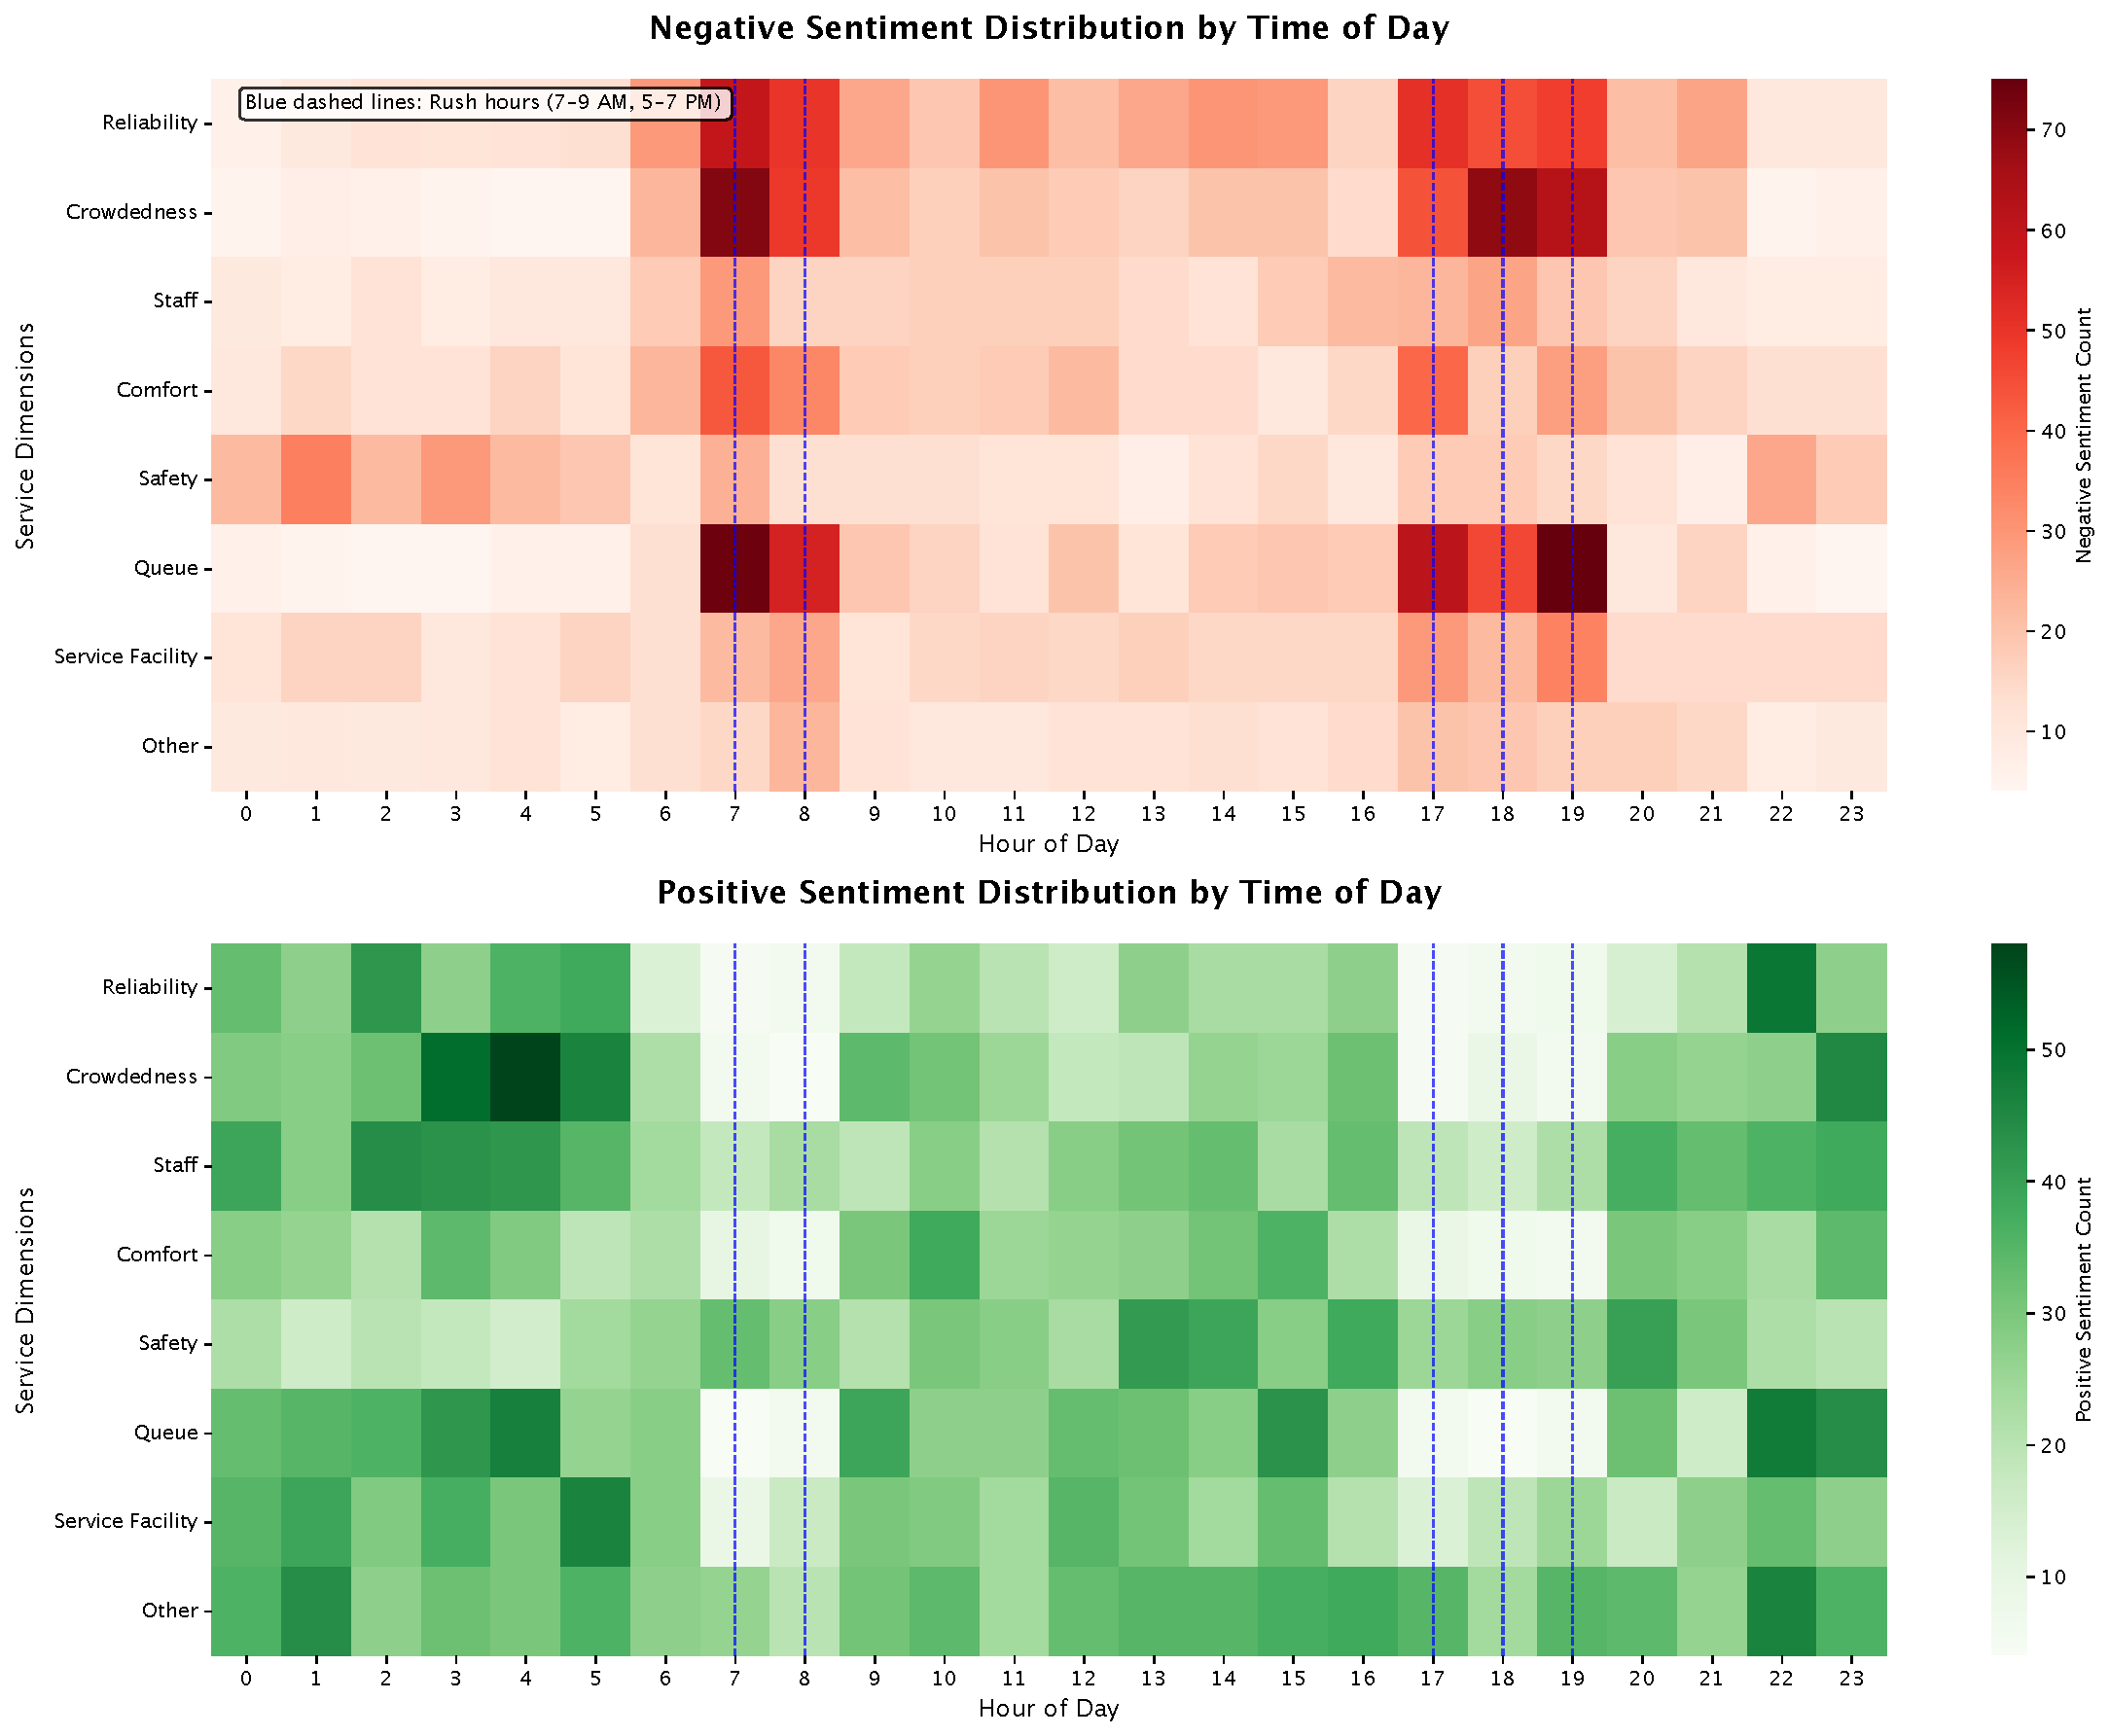
\includegraphics[width=0.99\textwidth]{figs/temporal_distribution_vis/time_of_day_sentiment_heatmap.pdf}
% \caption{Hourly sentiment heatmap analysis showing clear peak-hour negative sentiment patterns and improved satisfaction during off-peak periods}\label{fig:hourly_sentiment}
% \end{figure}

% \hyperref[fig:day_of_week_sentiment]{Fig.~\ref{fig:day_of_week_sentiment}} demonstrates clear weekly cyclical patterns, with negative sentiment consistently peaking on weekdays (Monday through Friday) and showing substantial reduction during weekends. This pattern reflects the commuter-dominated usage during workdays, where system stress and passenger frustration reach maximum levels.

% \begin{figure}[htbp]
% \centering
% 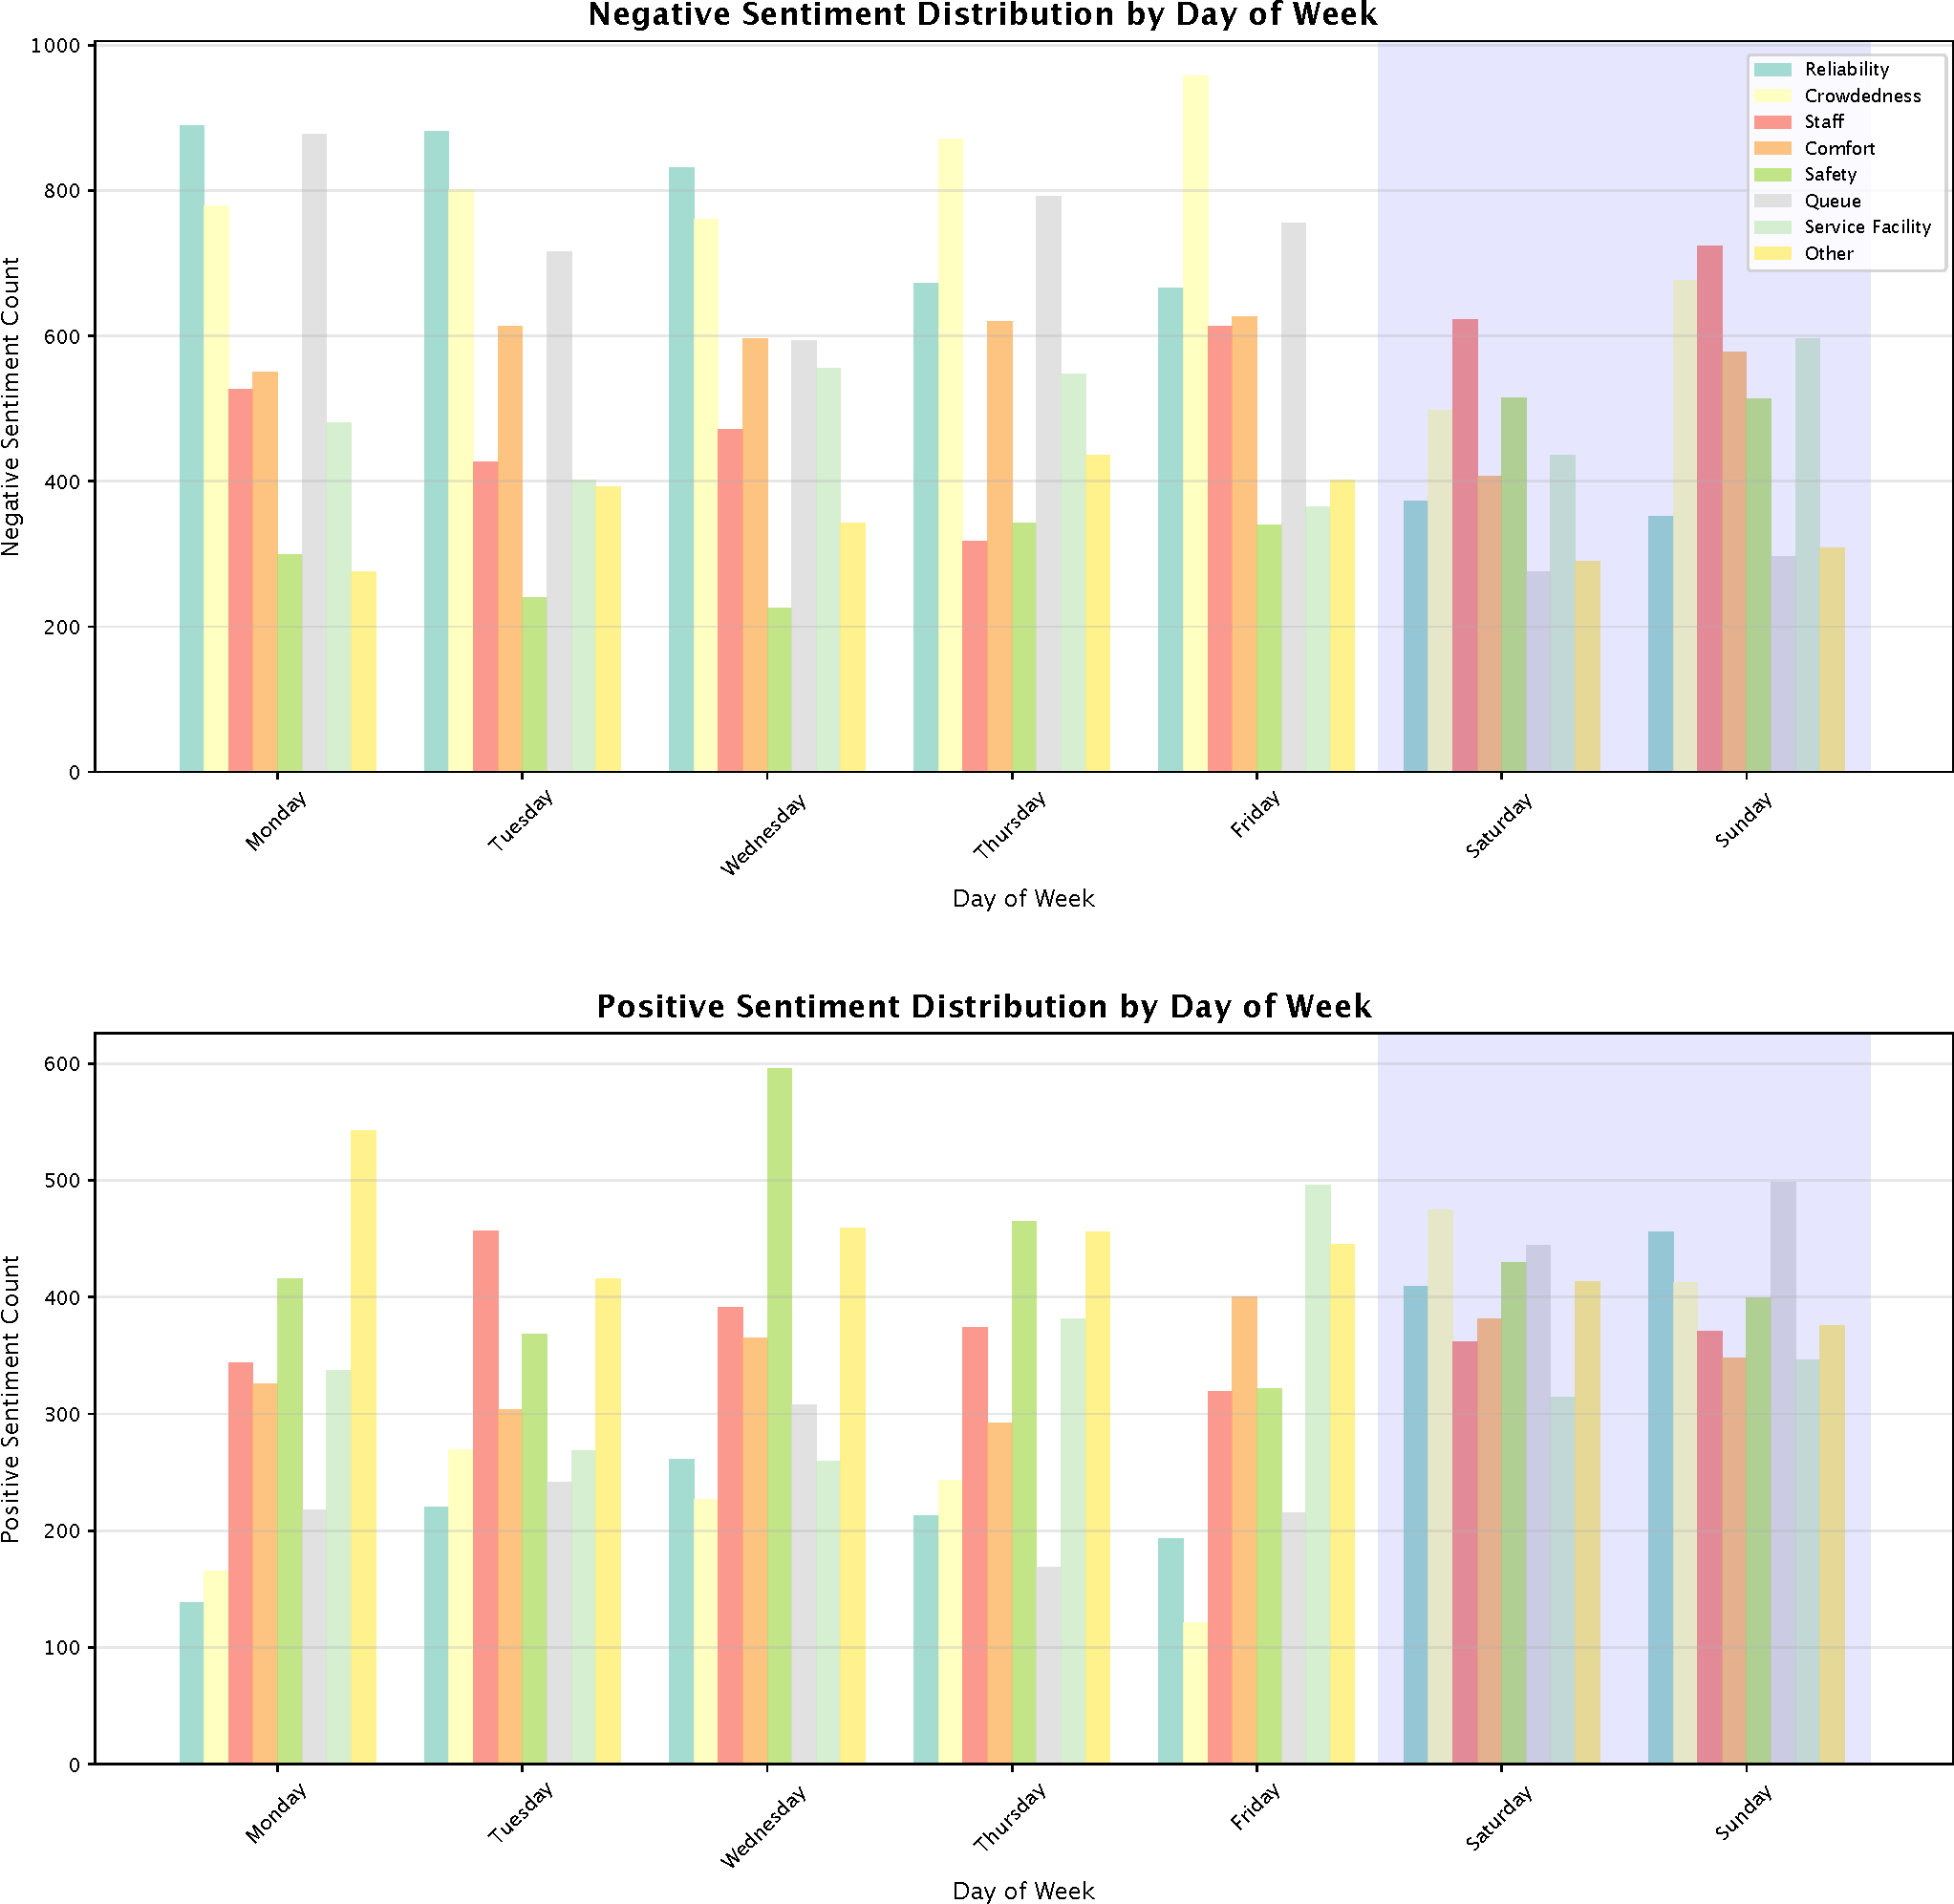
\includegraphics[width=0.99\textwidth]{figs/temporal_distribution_vis/day_of_week_sentiment_bars.pdf}
% \caption{Weekly sentiment distribution patterns showing higher negative sentiment during weekdays and improved satisfaction during weekends across all sentiment categories}\label{fig:day_of_week_sentiment}
% \end{figure}

% Monthly sentiment variations (\hyperref[fig:month_sentiment]{Fig.~\ref{fig:month_sentiment}}) reveal seasonal effects and long-term system performance trends. The analysis shows distinct seasonal patterns with increased negative sentiment during summer months (June-August), likely reflecting the impact of high temperatures and humidity on passenger comfort in underground environments. Conversely, winter months demonstrate relatively improved sentiment scores, suggesting better passenger experience during cooler weather conditions.

% \begin{figure}[htbp]
% \centering
% 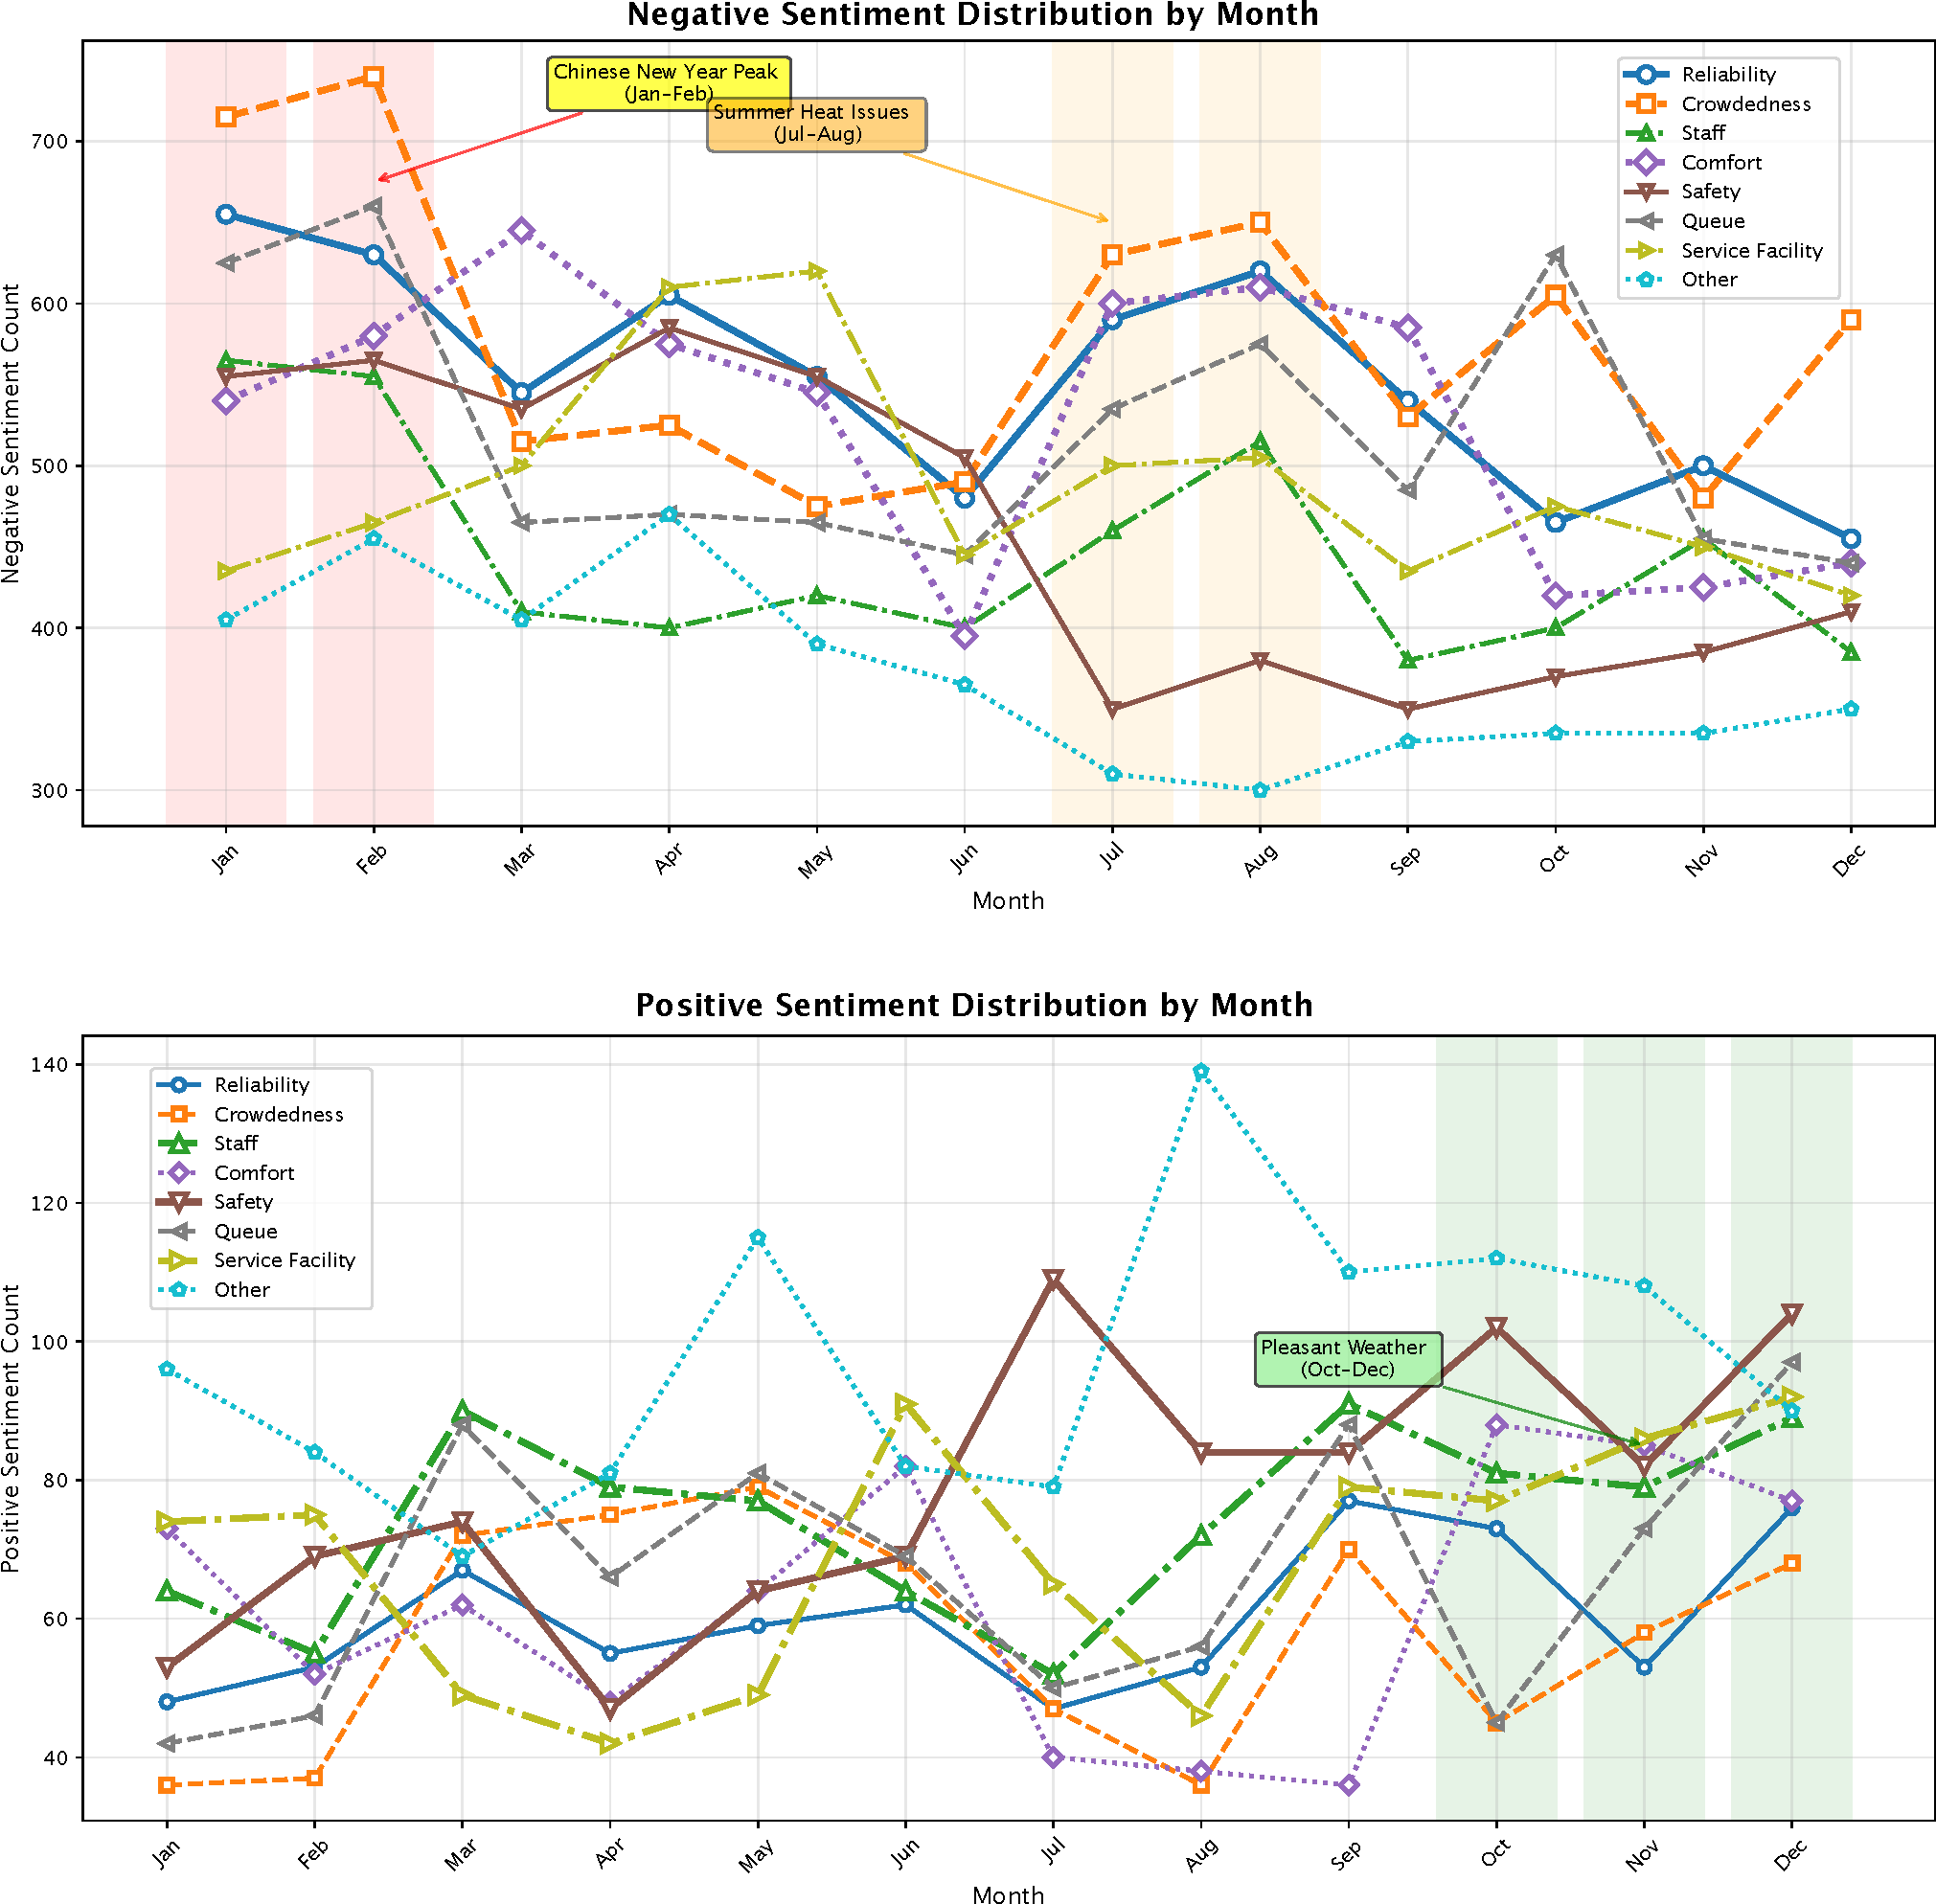
\includegraphics[width=0.99\textwidth]{figs/temporal_distribution_vis/month_of_year_sentiment_lines.pdf}
% \caption{Monthly sentiment trend analysis revealing seasonal variations and long-term performance patterns across different sentiment dimensions}\label{fig:month_sentiment}
% \end{figure}

\section{Conclusion}\label{sec:conclusion}
Evaluating passenger satisfaction is crucial for improving public transit, but leveraging social media data effectively faces significant challenges. Exsiting methods including general-purpose LLMs struggle with two key research gaps identified in this study: (1) the inability to accurately isolate genuine passenger feedback from incidental transit references in raw social media data, leading to unreliable analysis; and (2)the failure of conventional sentiment models to incorporate essential spatio-temporal context, resulting in poor performance in evaluating transit service quality. To address these gaps, this study introduces TranSenti, a novel framework specifically designed for transit satisfaction analysis. 

TranSenti has two primary contributions: it employs a hybrid filtering method that combines LLM-driven relevance scoring for semantic understanding, KL-divergence optimization to ensure consensus and reliability across multiple models, and instruction refinement for iterative domain-specific adaptation in identifying genuine transit feedback from raw social media posts. Second, TranSenti proposes a RoBERTa-based sentiment model enhanced with spatio-temporal fine-tuning to improve the sentiment analysis accuracy. 

Empirical evaluation using social media data related to the Shenzhen Metro system validates TranSenti's effectiveness. The hybrid filtering module considerably reduced filtering inaccuracies compared to keyword-based methods and other state-of-the-art benchmarks and showed that iterative optimization using KL-divergence and refining instructions significantly improved the ability of large language models (LLMs) to identify transit-related contexts. In sentiment classification, spatiotemporal RoBERTa reaches the F1 score of 80. 8\% and outperforms seven state-of-the-art benchmarks by margins between 6.2\% and 18.7\%.Ablation studies further confirmed the importance of contextual encodings, showing a 4. 9\% F1 score drop (to 75. 9\%) without the temporal encoder and an additional 2.4\% decline without the spatial encoder. These results highlight the necessity of grounding sentiment analysis in domain-specific operational knowledge, allowing transit authorities to differentiate between systemic and random issues.

Although our research shows the potential of TranSenti, several limitations must be acknowledged. First, the representativeness of our social media sample is subject to bias in demographic coverage. For example, social media data are reported to often overrepresent the opinions of young people and ignore those of other age groups \citep{de2017travel, abenoza2017travel}. Second, despite the strong understanding capabilities of advanced LLMs, issues such as hallucinations or occasional misinterpretations remain a concern and require further calibration and validation \citep{yao2023llm}. In future work, we plan to incorporate data from diverse sources, such as targeted surveys, which could provide a more comprehensive view of passenger satisfaction to reduce sampling bias \citep{nikolaidou2018utilizing}. Another way to improve sample representativeness is to develop re-weighting techniques for social media data based on known demographic distributions \citep{cui2021inferring}. Regarding LLM reliability, future studies could explore more advanced customized fine-tuning strategies in the transit domain, potentially incorporating human-in-the-loop systems for continuous model refinement and validation, or developing methods to quantify and reduce LLM uncertainty in this specific context \citep{yang2023human}. 

% \section*{Acknowledgement}

%Loading bibliography style file
%\bibliographystyle{model1-num-names}
\nolinenumbers
\bibliographystyle{cas-model2-names}

% Loading bibliography database
\bibliography{cas-refs}

% \section*{Appendix}
% Reliability and safety sentiments show distinct spatial patterns that reflect infrastructure quality and operational efficiency variations across the network. As illustrated in \hyperref[fig:reliability_negative]{Fig.~\ref{fig:reliability_negative}} and \hyperref[fig:safety_negative]{Fig.~\ref{fig:safety_negative}}, newer line segments and recently upgraded stations demonstrate significantly higher positive sentiment scores, while older infrastructure correlates with increased negative feedback regarding service reliability and safety concerns.

% \begin{figure}[htbp]
% \centering
% \includegraphics[width=0.48\textwidth]{figs/spatio_distribution_vis/shenzhen_metro_reliability_negative_sentiment_unified_normalized_heatmap.png}
% \includegraphics[width=0.48\textwidth]{figs/spatio_distribution_vis/shenzhen_metro_reliability_positive_sentiment_unified_normalized_heatmap.png}
% \caption{Spatial distribution of reliability-related sentiment: (left) negative sentiment in older network segments; (right) positive sentiment in newer infrastructure areas}\label{fig:reliability_negative}\label{fig:reliability_positive}
% \end{figure}

% \begin{figure}[htbp]
% \centering
% \includegraphics[width=0.48\textwidth]{figs/spatio_distribution_vis/shenzhen_metro_safety_negative_sentiment_unified_normalized_heatmap.png}
% \includegraphics[width=0.48\textwidth]{figs/spatio_distribution_vis/shenzhen_metro_safety_positive_sentiment_unified_normalized_heatmap.png}
% \caption{Spatial distribution of safety-related sentiment: (left) safety concerns concentrated in high-traffic interchange stations; (right) positive safety perceptions in well-maintained station areas}\label{fig:safety_negative}\label{fig:safety_positive}
% \end{figure}

% Service facility and staff-related sentiments (\hyperref[fig:service_facility_negative]{Fig.~\ref{fig:service_facility_negative}} and \hyperref[fig:staff_positive]{Fig.~\ref{fig:staff_positive}}) exhibit more dispersed spatial patterns, suggesting that service quality variations are less systematically correlated with geographical location and more dependent on local management practices and resource allocation.

% \begin{figure}[htbp]
% \centering
% \includegraphics[width=0.48\textwidth]{figs/spatio_distribution_vis/shenzhen_metro_service_facility_negative_sentiment_unified_normalized_heatmap.png}
% \includegraphics[width=0.48\textwidth]{figs/spatio_distribution_vis/shenzhen_metro_service_facility_positive_sentiment_unified_normalized_heatmap.png}
% \caption{Spatial distribution of service facility sentiment: (left) negative sentiment scattered across network; (right) positive sentiment showing variable facility quality}\label{fig:service_facility_negative}\label{fig:service_facility_positive}
% \end{figure}

% \begin{figure}[htbp]
% \centering
% \includegraphics[width=0.48\textwidth]{figs/spatio_distribution_vis/shenzhen_metro_staff_negative_sentiment_unified_normalized_heatmap.png}
% \includegraphics[width=0.48\textwidth]{figs/spatio_distribution_vis/shenzhen_metro_staff_positive_sentiment_unified_normalized_heatmap.png}
% \caption{Spatial distribution of staff-related sentiment: (left) negative sentiment distribution; (right) positive sentiment patterns reflecting service quality variations}\label{fig:staff_negative}\label{fig:staff_positive}
% \end{figure}


\end{document}